%:Clase del documento
\documentclass[fontsize=10pt, Myfinal=false, twoside, numbers=noenddot]{scrbook}
%Minion=true, English=true, Myfinal=true

%:Paquete de estilos original
\usepackage{libroETSI}

%:Paquete específico para cargar tikz (y sus librerías) y pgfplots
\usepackage{dtsc-creafig}

%:Paquete para notaciones específicas
\usepackage{notacion}

%:Paquete para incorporar aspectos concretos de la edición
\usepackage{edicionPFC}

\usepackage{indentfirst}

%:Espacio de una línea entre párrafos
\setlength{\parskip}{\baselineskip}

%:Evitar que LaTex corte las palabras.
\pretolerance=2000
\tolerance=3000

\newcommand{\bibhref}[3][blue]{\href{#2}{\color{#1}{#3}}}%

\AtBeginDocument{%
	\renewcommand\bibname{Referencias}
}

\newcommand\TODO[1]{\textcolor{red}{#1}}
%:\renewcommand\TODO[1]{} %PARA OCULTARLAS

%:Para modificar fácilmente la fuente del texto.
\makeatletter
\ifdtsc@Minion
\ifluatex
\setmainfont[Renderer=Basic, Ligatures=TeX,	% Fuente del texto 
Scale=1.01,
]{Minion Pro}
% En este caso conviene modificar ligeramente el tamaño de las fuentes matemáticas
\DeclareMathSizes{10}{10.5}{7.35}{5.25}
\DeclareMathSizes{10.95}{11.55}{8.08}{5.77}
\DeclareMathSizes{12}{12.6}{8.82}{6.3}
\fi
\else
\ifluatex
\setmainfont[Renderer=Basic, Ligatures=TeX, 
Scale=1.0,
]{Times New Roman}
\else
\usepackage{tgtermes}
\fi
\fi
\makeatother

\makeglossaries

%Lista de acrónimos para el glosario
\newacronym{SaaS}{SaaS}{software como servicio}
\newacronym{DevOps}{DevOps}{Development and Operations}
\newacronym{SW}{SW}{software}
\newacronym{QA}{QA}{Quality Assurance}
\newacronym{CI}{CI}{Continuous Integration}
\newacronym{TFM}{TFM}{Trabajo Fin de Máster}
\newacronym{SO}{SO}{Sistema Operativo}
\newacronym{OS}{OS}{Operative System}
\newacronym{TI}{TI}{Tecnología de la información}
\newacronym{CVE}{CVE}{Common Vulnerabilities and Exposures}
\newacronym{IC}{IC}{Integración continua}
\newacronym{API}{API}{Interfaz de Programación de Aplicaciones}

%\href{https://jenkins.io/}{Jenkins}

% Formato A4
\geometry
{paperheight=297mm,%
	paperwidth=210mm,%
	top=25mm,%
	headsep=8.5mm,%
	includefoot, 
	textheight=240mm, 
	textwidth=150mm, 
	bindingoffset=0mm, 
	twoside}

\usepackage[a4,center]{crop}%para poner las cruces de esquina de página, poner la opción cross

%:Esquema de numeración por defecto
\setenumerate[1]{label=\normalfont\bfseries{\arabic*.}, leftmargin=*, labelindent=\parindent}
\setenumerate[2]{label=\normalfont\bfseries{\alph*}), leftmargin=*}
\setenumerate[3]{label=\normalfont\bfseries{\roman*.}, leftmargin=*}
\setlist{itemsep=.1em}
\setlength{\parindent}{1.0 em}

% El nivel hasta el que se muestra el índice 
\setcounter{tocdepth}{1}

%:Empieza el documento

\begin{document}
	
	%:Para incluir toda la referencia bibliográfica aunque no se cite, descomente la siguiente línea
	%:\nocite{*}
	
	%:Inicio de la portada
	
	%:Para crear la portada y la portada interior (pagina titular)
	\titulo{Seguridad en la integración continua de la metodología ágil y la filosofía DevOps} %\mbox evita que se divida una palabra al cambiar de línea
	\autor{Eleazar Rubio Sorrentino}
	\director{Juan Manuel Vozmediano Torres}
	\titulodirector{Profesor Titular}
	
	\departamento{Dep. de Ingeniería Telemática}
	\centro{Escuela Técnica Superior de Ingeniería}
	\universidad{Universidad de Sevilla}
	\titulacion{Ingeniería de Telecomunicación}
	\fecha{2017}
	\nombretrabajo{Trabajo Fin de Máster}
	
	\hypersetup
	{
		linkcolor=black, %Enlaces en color negro.
		pdfauthor={\elautor},
		pdftitle={\nombretrabajo,\eltitulo}, 
		pdfkeywords={Latex, edición, formato de texto}	
	}
	
	%:logo de la Universidad y logo del departamento.
	\portadaPFC{figuras/LogoUS.pdf}{figuras/LogoIT.pdf}
	
	%:Fin de la portada
	
	%:Todo lo que constituye la primera parte del libro que no es el cuerpo del libro en realidad
	\frontmatter
	%:Pone la numeración en mayúscula (al menos en español).
	\pagenumbering{Roman}
	
	%!TEX root =../MemoriaTFM.tex
\chapter*{Agradecimientos}
%\pagestyle{especial}
\pagestyle{empty}
%\chaptermark{Agradecimientos}
\phantomsection
%\addcontentsline{toc}{listasf}{Agradecimientos}
%\vspace{1cm}
%{\huge{Agradecimientos}}
%\vspace{1cm}

\lettrine[lraise=-0.1, lines=2, loversize=0.25]{A}{unque} el trabajo aquí realizado pueda llevar al engaño por su propia definición, Trabajo \textit{Fin} de Máster, nada más lejos de la realidad, ya que esta etapa que ahora parece concluir, para mi no ha sido más que el principio y no ha hecho más que comenzar.

Creo que no desvarío si afirmo (rotundamente) que el Máster que aquí acaba ha sido el comienzo a mi nueva vida: nueva profesión, nueva ciudad, en un nuevo país, nuevos amigos, un número incontable de vuelos de ida y vuelta y un sin fin de nuevas experiencias, emociones y sensaciones que me dieron un fuerte empujón fuera de mi bien establecida \textit{zona de confort} (o así la llaman). 

"Al César lo que es del César" y hasta aquí lo que le pertenece. 

Lo cierto es que todo lo que ha provocado el haberme atrevido a seguir estudiando, después de una carrera tan larga, y todos los cambios y nuevas etapas que ha traído este Máster de la mano no tiene un sólo culpable al que dar las gracias, sino más bien varios.

Gracias a mi familia, a toda al completo, y no son pocos. Tengo la suerte de tener una gran familia que me apoya, me quiere, me comprende y cuida de mi por muy lejos o muy cerca que me encuentre, sabiendo siempre sacar lo mejor de mi. Diría que os debo la vida, pero es obvio.

Gracias a mi novia Eva, por ser como es, sin más. porque su amor infinito y su apoyo incondicional me hacen querer ser mejor persona cada día.

Gracias a mi amigo Pablo, porque si el que tiene un amigo tiene un tesoro, mi tesoro no tiene precio.

Gracias a Sergio, mi nuevo maestro de profesión, porque su paciencia y esfuerzo conmigo no tiene límites y por ser la persona que con ilusión "maquinó" la idea de la que ha surgido este Trabajo Fin Máster.

Y gracias a todas aquellas personas que confiaron en mi, ofreciéndome la oportunidad de crecer personal y profesionalmente, ¡No pienso desaprovecharla!. 

Esto no es más que el principio.

{\flushleft{\hfill \emph{Eleazar Rubio Sorrentino}}}%
\vspace{-.3cm}
{\flushleft{\hfill \emph{Sevilla, 2017}}}%
	
	%!TEX root =../MemoriaTFM.tex
\chapter*{Resumen}
\pagestyle{especial}
\chaptermark{Resumen}
\phantomsection
\addcontentsline{toc}{listasf}{Resumen}

\lettrine[lraise=-0.1, lines=2, loversize=0.2]{E}{n} los últimos tiempos de las empresas dedicadas al desarrollo de \gls{SaaS}, los conceptos de metodología ágil y la filosofía \gls{DevOps} están cobrando, cada vez más, un papel fundamental para el desarrollo de las mismas\cite{consultorit2017}. Según un estudio de alcance mundial realizado recientemente por CA Technologies, más del 75 por ciento de las organizaciones españolas coinciden en que las metodologías ágiles y \gls{DevOps} son cruciales para el éxito de la transformación digital\cite{catechnologies2017}.

Este nuevo modo de entender el mundo del desarrollo de \gls{SW} posee una serie de elementos comunes, cada uno de ellos implementado con herramientas cada vez más conocidas y populares para las empresas que lo llevan a la práctica: 

\begin{itemize}
	\item Plataformas de desarrollo colaborativo y control de versiones de \gls{SW} (por ejemplo GitHub\cite{github2017}), donde se almacena el código desarrollado por las mismas.
	\item Diferentes entornos o infraestructuras de trabajo para los desarrolladores, que van a permitir un desarrollo y despliegue continuo para las mejoras del producto: entornos de desarrollo, entornos de seguro de calidad o \gls{QA}, preproducción, producción o entorno final, etc.
	\item Fundamentos de \gls{IC} y \gls{DC}.
	\item Desarrollo y  de aplicaciones inmutables que utilizan contenedores de imágenes (generalmente de Docker\cite{docker2017}) para incrementar la protabilidad, reusabilidad y escalabilidad de la aplicación. Estas aplicaciones suelen mantener sus plataformas soportadas en Proveedores Cloud tales como \gls{AWS}\cite{aws2017}, Microsoft Azure\cite{azure2017} o \gls{GCE}\cite{google2017}.
\end{itemize}

El presente \gls{TFM} pretende exponer un proceso automatizado de análisis estático de aplicaciones en varios niveles. El resultado de la ejecución periódica de estos procedimientos genera informes de seguridad que podrán ser utilizados para prevenir amenazas durante las fases más tempranas del \gls{CDS} del software, advirtiendo de aspectos tales como:

\begin{enumerate}
	\item Si la aplicación creada tiene Vulnerabilidades (\gls{CVE}\cite{cve2017}) en las librerías de dependencias de código utilizadas.
	\item Si la imagen que se va a emplear para desplegar el contenedor de dicho \gls{SW} contiene vulnerabilidades conocidas al nivel de \gls{SO}.
\end{enumerate}

\chapter*{Abstract}
\pagestyle{especial}
\chaptermark{Abstract}
\phantomsection
\addcontentsline{toc}{listasf}{Abstract}

\lettrine[lraise=-0.1, lines=2, loversize=0.2]{L}{ately} inside Software as a Service (\gls{SaaS}) companies, the agile methodology and \gls{DevOps} philosophy concepts are taking a fundamental role for the development of them\cite{consultorit2017}. According to a recent global survey by CA Technologies, more than 75 percent of Spanish organizations agree that DevOps and agile methodologies are crucial to the success of digital transformation\cite{catechnologies2017}.

This new way of understanding the world of \gls{SW} development has various common elements, each of them implemented with well known and popular tools for the companies that put it into practice:

\begin{itemize}
\item Collaborative development platforms and \gls{SW} version control systems (for example GitHub\cite{github2017}), where the code developed is keeped.
\item Different environments and infrastructures for developers, which will allow to continuous development and deployment for product enhancements: development environments, Quality Assurance \gls{QA} environments, pre-production, production or final environment, etc.
\item \gls{CI} and \gls{CD} principles.
\item Deployment and orchestration of immutable application images using containers (mostly Docker) that increases the portability, reusability and scalability of the application. These applications use Cloud Providers as the underlaying platform such as \gls{AWS}\cite{aws2017}, Microsoft Azure\cite{azure2017} or \gls{GCE}\cite{google2017}.
\end{itemize}

This thesis tries to expose a procedure to automatically implement an application static analysis pipeline at several layers. The outcome of these periodically executed pipelines provide the company security reports that can be used to prevent threats during the earliest stages of the \gls{SDLC}:

\begin{enumerate}
\item If the application created has Vulnerabilities (\gls{CVE}\cite{cve2017}) in the code dependencies used.
\item If the image used to deploy the container of the mentioned \gls{SW} contains known vulnerabilities at the \gls{OS} level.
\end{enumerate}


	
	%:Índice
	\cleardoublepage
	\phantomsection
	\pagestyle{especial}
	\tableofcontents
	
	%:Empieza el contenido del libro
	\mainmatter
	
	%:Página por defecto
	\pagestyle{esitscCD}
	
	%:Los diferentes capítulos, en carpetas separadas
	
	%!TEX root =../MemoriaTFM.tex
%El anterior comando permite compilar este documento llamando al documento raíz
\chapter{Introducción}\label{chp-01}
\epigraph{You can ask 10 people for a definition of DevOps and likely get 10 different answers.}{Dustin Whittle, 2014\\Developer Advocate at Uber Developer Platform}

\lettrine[lraise=-0.1, lines=2, loversize=0.2]{E}{n} este primer apartado de la memoria se pretende realizar con el lector un recorrido a través del contexto que ha motivado el desarrollo del presente \gls{TFM} para el Máster en Seguridad de la Información y las Comunicaciones  de la Universidad de Sevilla, con el fin de aclarar el objetivo perseguido en su realización. Como conclusión al mismo, se definirá la estructura seguida durante la redacción, introduciendo cada uno de los apartados que se encontrarán a continuación. 

\section{Contexto y motivación}

El año 2017, para empresas englobadas en todo tipo de sectores, está siendo el año de la transformación digital. Estos procesos de transformación exigen distintas formas de trabajo, más ágiles y colaborativas, con las que poder aplicar nuevas tecnologías que permitan conseguir los objetivos del negocio, en entornos que afrontan grandes desafíos culturales, organizativos y operativos e incluso pueden llegar a tener que lidiar con sistemas tecnológicos antiguos y casi obsoletos\cite{expansion2017}. 

Es en este contexto donde el concepto \gls{DevOps} empieza a sonar con más fuerza: el contexto de las metodologías ágiles. 

De esta forma, \gls{DevOps} es un concepto de trabajo, basada en el desarrollo de código, que usa nuevas herramientas y prácticas para reducir la tradicional distancia entre técnicos de programación y de sistemas, respondiendo a la necesidad experimentada por el sector tecnológico de dar una respuesta más rápida a la implementación y operación de aplicaciones. Este nuevo enfoque de colaboración que es \gls{DevOps} permite a los equipos trabajar de forma más cercana, aportando mayor agilidad al negocio y notables incrementos de productividad.

Desde las pruebas de concepto hasta el lanzamiento, pasando por el \textit{testing} y los entornos de prueba, todos los pasos involucrados requieren de la máxima agilidad posible (\autoref{proceso-DevOps}), y eso pasa por integrar los procesos y los equipos de programación con los de sistemas\cite{claranet2017}.

\begin{figure}[htbp]
	\centering
	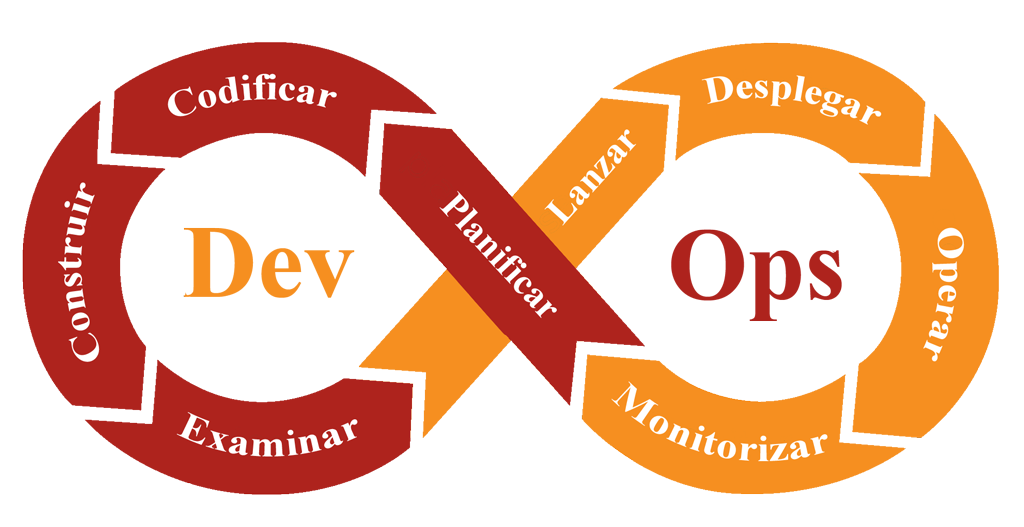
\includegraphics[width=0.80\linewidth]
	{introduccion/figuras/proceso-devops.png}
	\caption{Introducción al proceso DevOps}
	\label{proceso-DevOps}
\end{figure}

Por otro lado, el concepto de contenedor de aplicación (aislamiento de espacio de nombres y gobernanza de recursos) a pesar de no ser un concepto novedoso, está cobrando cada vez más y más relevancia en el panorama de la empresa actual, de la mano de las continuas mejoras que experimentan las tecnologías que lo implementan, simplificando la administración y transformando la forma en que se desarrolla, distribuye y ejecuta el software, en forma de microservicio\footnote{Aproximación para el desarrollo software que consiste en construir una aplicación como un conjunto de pequeños servicios, los cuales se ejecutan en su propio proceso y se comunican con mecanismos ligeros (normalmente una API de recursos HTTP)}, además de proveer la habilidad de encapsular todo el entorno utilizado con el objetivo de ser desplegado en los sistemas de producción de la empresa, manteniendo las mismas características, aumentando la escalabilidad y disminuyendo notablemente los costes asociados a infraestructuras.

Los contenedores juegan un papel clave en un entorno \gls{DevOps} porque soportan las implementaciones de la pila de desarrollo y operaciones completa y van en camino de formar parte de la definición básica de lo que se conocerá como \gls{DevOps} en unos pocos años\cite{searchdatacenter2015}.

Además, la metodología \gls{DevOps} representa una gran promesa a la hora de asegurar el desarrollo del software, ya que las organizaciones pueden potencialmente encontrar y remediar las vulnerabilidades con mayor frecuencia y al principio del ciclo de vida de la aplicación, ahorrando costes y tiempo. Conforme al informe de  \textit{"Seguridad de Aplicaciones y DevOps"} de octubre de 2016 promovido por Hewlett Packard Enterprise\cite{hpe2016}, que incluye tanto respuestas cualitativas como cuantitativas de profesionales de operaciones informáticas, líderes de seguridad y desarrolladores, se concluye que el 99\% de los encuestados confirma que la adopción de la cultura \gls{DevOps} aporta la oportunidad de mejorar la seguridad de las aplicaciones. Sin embargo, solo el 20\% realizan análisis de seguridad de aplicaciones durante el desarrollo y el 17\% no utilizan ninguna tecnología que proteja sus aplicaciones, destacando una desconexión significativa entre la percepción y la realidad de la seguridad \gls{DevOps}.

Es en el contexto planteado donde surge la idea del presente \gls{TFM}: aportar mecanismos a la metodología \gls{DevOps} que permitan analizar la seguridad de las aplicaciones desarrolladas y el contenedor que las albergará dentro de la infraestructura de la empresa, sin interferir de manera destructiva con el propio proceso de desarrollo y depliegue de la aplicación.

\section{Objetivo}

El objetivo del presente Trabajo Fin de Máster (\gls{TFM}) es desarrollar un entorno, basado en contenedores, que pueda ser incluido en el proceso de desarrollo e integración continua de la empresa y con el que poder realizar tareas periódicas programadas para analizar estáticamente las posibles vulnerabilidades de seguridad contenidas en las dependencias de aplicaciones desarrolladas mediante los lenguajes de programación Ruby y NodeJS, por ser dos de los lenguajes de programación más utilizados en el desarrollo de aplicaciones Web, además de analizar a nivel del \gls{SO} vulnerabilidades presentes en las imágenes que van a constituir el contenedor que dará soporte a dichas aplicaciones.

Como medio para alcanzar el objetivo planteado se va a hacer uso de una serie de aplicaciones y herramientas, entres las que cabe destacar las siguientes, que serán desarrolladas en los próximos apartados:

\begin{itemize}
	\item GitHub\cite{github2017}: Plataforma de desarrollo colaborativo y control de versiones de \gls{SW} donde almacenar, entre otras, el código desarrollado y que será analizado.
	\item Jenkins \gls{CI}\cite{jenkins2017}: Software de Integración Continua (\gls{IC}) con el que automatizar los trabajos periódicos de análisis estático a realizar.
	\item Docker\cite{docker2017}: Proyecto de código abierto que automatiza el despliegue de aplicaciones dentro de contenedores de software, con el que desplegar los distintos elementos requeridos.
\end{itemize}

El trabajo aquí presentado no tiene como objetivo innovar en la tecnología existente, sino por contra valerse de esta para aportar al futuro usuario una herramienta intuitiva y de fácil aplicación, resultado de la agrupación de otras utilidades, con la que poder desplegar con el mínimo esfuerzo el entorno aquí recopilado. 

\section{Estructura de la memoria}


Para facilitar la lectura de la memoria actual, se cree conveniente presentar un resumen de cómo se estructuran los diferentes apartados que contiene.

En el apartado actual, Introducción, se presenta el \gls{TFM} que se va a realizar, aclarando el objetivo perseguido, el contexto en que surge y los aspectos que motivaron su realización.

El apartado \ref{chp-02}, Descripción de la técnica, pretende dar a conocer, de manera objetiva, las características de la realidad representada, con rasgos tales como elementos que la componen, utilidad, etc. En concreto, el apartado comienza describiendo en qué consiste la metodología Ágil, los mecanismo o procesos de Integración Continua \gls{IC} y Despliegue Continuo \gls{DC}, así como el Ciclo de Desarrollo Seguro de software (\gls{SDLC}). Para concluir el apartado se aclarará al lector en qué consiste un análisis estático y qué es lo que se conoce como virtualización basada en contenedores.

El apartado \ref{chp-03}, Entorno de trabajo, está dedicado a conocer las herramientas utilizadas para poder llevar a cabo el desarrollo y la implementación de la parte técnica de este \gls{TFM}.

El apartado \ref{chp-04}, titulado Desarrollo de la aplicación, es el apartado principal de la memoria. En él, se detalla el proceso a seguir durante el desarrollo e implementación de los objetivos presentados en este proyecto, comenzando con la preparación del entorno que se va a utilizar en el desarrollo, hasta llegar a presentar el Resultado final obtenido como conclusión al proceso de desarrollo del sistema.

Por último, el apartado \ref{chp-05}, está dedicado a las Conclusiones y evaluaciones surgidas del proyecto, los objetivos alcanzados y las líneas futuras de trabajo surgidas durante la realización de éste.

\endinput

	
	%!TEX root =../MemoriaTFM.tex
%El anterior comando permite compilar este documento llamando al documento raíz
\chapter{Descripción de la Técnica}\label{chp-02}
\epigraph{A good DevOps organization will free up developers to focus on doing what they do best: write software. }{Rob Steward, 2015\\Global Vicepresident at Verint-Systems.}

\lettrine[lraise=-0.1, lines=2, loversize=0.2]{P}{ara} comprender el desarrollo del trabajo aquí presentado, tal y como se ha llevado a cabo, se debe conocer la situación en que éste se desarrolla, la tecnología de la que se dispone y los elementos existentes y necesarios, de una manera objetiva.

Es por esto, que el apartado actual está orientado a conocer las características de la realidad representada y a introducir las bases tecnológicas del presente \gls{TFM}, resaltando los conceptos más importantes.

\section{Empresas \gls{TI}}

\TODO{Pipelines y demás en empresas modernas... ¿Cómo se hacen las cosas? y comentar de qué forma no se va a interferir de manera destructiva en este proceso... y quizás esto último en otro apartado... ¿Incluyo aquí cómo puede ser "más o menos" un día de trabajo DevOps?}

\section{Integración Continua \gls{IC}}

(Continuous Integration, \gls{CI})
(Software de) 

\section{CVE}

\TODO{Breve muy breve}

\section{Análisis estático}



\subsection{Ruby y NodeJS}

\TODO{YAML no e stá por ningún lado.}

Quizás a estas alturas no sea necesario hablar de estos lenguajes de programación... lo que si que daré será algunos datos que confirmen un poco por qué he empezado con estos...

\TODO{Breve presentación a la importancia de estos lenguajes de programación, comentando que lo que se ha hecho aquí es extensible a otros lenguajes, con otras herramientas similares.\\Concepto dependencias de código.}

Bundler is the de facto way of managing dependencies. It provides, among other things, a clear way of specifying required libraries and their versions, by keeping track of everything for you through Gemfile and (for applications) Gemfile.lock. Exactly the sort of information you’d need when checking for security vulnerabilities.

\subsection{De las dependencias del código}

\TODO{¿Qué es y cómo funciona?}

\subsection{De contenedores de imágenes}

\TODO{Quizás no son necesarios los subapartados... y simplemente baste con explicar elconcepto de análisis estático de algo genérico.}

https://www.linuxadictos.com/docker-i-que-es-conociendo-la-ballena.html

http://www.javiergarzas.com/2015/07/que-es-docker-sencillo.html

https://www.redeszone.net/2016/02/24/docker-funciona-la-virtualizacion-contenedores/


La nube es cada vez más grande, más potente, cuenta con más usuarios que hacen uso de ella al mismo tiempo y, además, permite la ejecución de aplicaciones cada vez más potentes, por lo que, para garantizar el correcto funcionamiento de esta, tanto en el presente como en el futuro, es necesario utilizar una plataforma que optimice los recursos lo mejor posible y, al mismo tiempo, sea lo más escalable posible con el fin de poder ampliar sus características de forma sencilla cuando sea necesario.

La nube es sinónimo de virtualización. Ejecutar un sistema operativo virtual por cada instancia de una aplicación es un proceso muy pesado y poco optimizado, a la vez que lento. Por ello, la comunidad Linux ha trabajado en el concepto de contenedores, una nueva forma de optimizar recursos creando pequeños espacios virtuales de las aplicaciones necesarias cargando solo el núcleo de la aplicación y las dependencias, pero funcionando siempre sobre un único kernel, o sistema operativo. (Esquema de esta WEB)

\section{Trabajos relacionados}

\endinput
	
	%!TEX root =../MemoriaTFM.tex
%El anterior comando permite compilar este documento llamando al documento raíz
\chapter{Entorno de trabajo}\label{chp-03}
\epigraph{Technology is nothing. What's important is that you have a faith in people, that they're basically good and smart, and if you give them tools, they'll do wonderful things with them.}{Steve Jobs, 1994\\Businessman}

\lettrine[lraise=-0.1, lines=2, loversize=0.2]{A}{ntes} de comenzar el proceso de desarrollo de la aplicación es necesario preparar un entorno adecuado de trabajo, es decir, un conjunto de herramientas hardware y software que permitan llevar a cabo el proyecto con la mayor comodidad y precisión posible.

La correcta elección de un entorno de trabajo adecuado es fundamental a la hora de abordar cualquier tipo de proyecto, ya que el éxito o fracaso, o al menos la eficiencia del proceso de desarrollo del mismo, va a depender en gran medida de dicho entorno utilizado.
El apartado actual presenta el entorno de trabajo utilizado para la realización de este \gls{TFM}.

\section{Git y GitHub}

Los sistemas de control de versiones son programas cuyo principal objetivo es controlar los cambios producidos en el desarrollo de cualquier tipo de software, permitiendo conocer el estado actual de un proyecto, las personas que intervinieron en ellos, etc. Un buen control de versiones es tarea fundamental para la administración de un proyecto de desarrollo de software en general\cite{alcazar2014}. Git es uno de los sistemas de control de versiones más populares entre los desarrolladores, es gratuito, open source, rápido y eficiente, aunque gran parte su popularidad es debido a GitHub(\autoref{jenkins-logo}), un excelente servicio de alojamiento de repositorios de software que ofrece un amplio conjunto de características de gran utiilidad para el trabajo en equipo.

\begin{figure}[htbp]
	\centering
	
\includegraphics[width=0.80\linewidth]
	{entorno/figuras/github.png}
	\caption{Logotipo de GitHub}
	\label{github-logo}
\end{figure}

A continuación se muestran algunas de las características que han llevado a GitHub a ser tan valorado entre los desarrolladores\cite{quintana2015}:

\begin{itemize}
	\item Permite versionar el código, es decir, guardar en determinado momento los cambios realizados sobre un archivo o conjunto de archivos con la oportunidad de tener acceso al historial de cambios al completo, bien para regresar a alguna de las versiones anteriores o bien para poder realizar comparaciones entre ellas.
	\item Gracias a la gran cantidad de repositorios de \gls{SW} públicos que alberga, es posible leer, estudiar y aprender de el código creado por miles de desarrolladores en el mundo, permitiendo incluso la oportunidad de adaptarlos a las necesidades propias de cada desarrollador, sin alterar el original y realizando una copia o fork\footnote{Copia exacta en crudo del repositorio original que podrá ser utilizada como un repositorio git cualquiera} de este.
	\item Tras haber realizado un fork de un proyecto y haber realizado algunos ajuste, introducido alguna mejora o arreglado algún problema que este pudiera contener, es posible integrar los cambios realizados al proyecto original (previa supervisión de su propietario, administrador o alguno de sus colaboradores), por lo que un repositorio puede llegar a ser construido mediante la contribución una gran comunidad de desarrolladores.
	\item GitHub posee un sistema propio de notificaciones con el que poder estar informado de lo que ocurre en torno a un repositorio concreto, ya sea privado a la compañía o público a la comunidad.
	\item GitHub trae incorporado un visor de código, mediante el cual (y a través del navegador) es posible consultar el contenido de un archivo determinado, con la sintaxis correspondiente al lenguaje utilizado y sin necesidad de descargar una copia del mismo.
	\item Cada repositorio de \gls{SW} albergado en GitHub cuenta con su propio seguimiento de incidencias, con un elaborado sistema de tickets, de manera tal que cualquier colaborador (o usuario en general) pueda reportar algún problema encontrado en la utilización el código o pueda simplemente sugerir nuevas características para que sean implementadas.
	\item Al ser una plataforma web es totalmente independiente al \gls{SO} utilizado, siendo por otro lado Git compatible con los principales sistemas actuales: Linux, Windows, OSX.
	\item GitHub es gratuito e ilimitado para repositorios de proyectos públicos, sólo aquellos usuarios que deseen mantener proyectos en privado deberán pagar una cuota. 
\end{itemize}

\TODO{TODO - Una frase de cierre al apartado}


\section{bundler-audit}

Como ya fue comentado en el apartado \ref{chp-02} cada aplicación tiene sus dependencia, y estas a su vez pueden contener vulnerabilidades de seguridad. Encontrar las vulnerabilidades de seguridad que presenta una aplicación es una tarea necesaria y tediosa, que de ser obviada no impedirá que la aplicación generada siga siendo ejecutada como si todo estuviera funcionando en perfectas condiciones, pero que ocultará agujeros en la aplicación que podrán ser utilizados en diversa manera por algún usuario malintencionado.

Para cualquier aplicación escrita con Ruby y en ausencia de alguna herramienta automatizada de análisis de vulnerabilidades, el desarrollador del código deberá estar suscrito a cada lista de correo relacionada con anuncios de seguridad de dependencias y realizar un seguimiento exclusivo de vulnerabilidades y actualizaciones de seguridad de cada una de las dependencias incluidas en la aplicación, para cada aplicación en la que participe\cite{prescott2015}.

Por el contrario, todo este proceso puede ser automatizado en Ruby gracias a bundler-audit\cite{bundleaudit2017}del grupo de colaboradores Rubysec, un verificador a nivel de parche para Bundler con las siguientes características:

\begin{itemize}
	\item bundler-audit analiza las vulnerabilidades en las versiones de las gemas contenidas en el archivo de dependencias \textit{Gemfile.lock} de la aplicación.
	\item Analiza las fuentes de dependencias que puedan ser inseguras (http://).
	\item Permite especificar avisos de seguridad que serán ignorados en el análisis, bien por ser un riesgo asumido por el desarrollador, una vulnerabilidad ya conocida y en la que se está actualmente trabajando o cualquier otro motivo.
	\item No requiere de conexión a internet para cada ejecución que se realice del análisis.
	\item Funcionando cruzando la información de dependencias recogidas del fichero \textit{Gemfile.lock} con una lista de vulnerabilidades conocidas\cite{advisorydb2017}, basada en información pública existente en bases de datos como \gls{CVE}.
\end{itemize}

El código \ref{prg03-01} muestra un ejemplo del resultado obtenido a la salida del terminal de comandos al realizar un análisis estático de vulnerabilidades con bundler-audit al archivo \textit{Gemfile.lock} de un proyecto:

\begin{lstlisting}[language=,caption={Ejemplo de uso de bundler-audit}, breaklines=true, label=prg03-01]
$ bundle audit
Name: actionpack
Version: 3.2.10
Advisory: OSVDB-91452
Criticality: Medium
URL: http://www.osvdb.org/show/osvdb/91452
Title: XSS vulnerability in sanitize_css in Action Pack
Solution: upgrade to ~> 2.3.18, ~> 3.1.12, >= 3.2.13

Name: actionpack
Version: 3.2.10
Advisory: OSVDB-89026
Criticality: High
URL: http://osvdb.org/show/osvdb/89026
Title: Ruby on Rails params_parser.rb Action Pack Type Casting Parameter Parsing Remote Code Execution
Solution: upgrade to ~> 2.3.15, ~> 3.0.19, ~> 3.1.10, >= 3.2.11

Name: activerecord
Version: 3.2.10
Advisory: OSVDB-90072
Criticality: Medium
URL: http://direct.osvdb.org/show/osvdb/90072
Title: Ruby on Rails Active Record attr_protected Method Bypass
Solution: upgrade to ~> 2.3.17, ~> 3.1.11, >= 3.2.12

Name: activerecord
Version: 3.2.10
Advisory: OSVDB-89025
Criticality: High
URL: http://osvdb.org/show/osvdb/89025
Title: Ruby on Rails Active Record JSON Parameter Parsing Query Bypass
Solution: upgrade to ~> 2.3.16, ~> 3.0.19, ~> 3.1.10, >= 3.2.11

Unpatched versions found!
\end{lstlisting}

Además, bundler-audit permite actualizar la base de datos ruby-advisory-db yanalizar el fichero \textit{Gemfile.lock} desde el mismo comando, habilidad que resulta de gran utilidad para su ejecución en sistemas de \gls{IC}, como muestra el código \ref{prg03-02}:

\begin{lstlisting}[language=,caption={Ejecutando bundler-audit tras la actualización de las vulnerabilidades conocidas}, breaklines=true, label=prg03-02]
$ bundle audit check --update
\end{lstlisting}

Por último, y como ya se ha mencionado con anterioridad en este apartado, es posible ignorar advertencias especificadas (código \ref{prg03-03}) por el usuario:

\begin{lstlisting}[language=,caption={Ignorar vulnerabilidades con bundler-audit}, breaklines=true, label=prg03-03]
$ bundle audit check --ignore OSVDB-108664
\end{lstlisting}


\TODO{TODO - Cierre del apartado. de Rubysec para proyectos Ruby}

\section{nsp}

de Node Security Platform para proyectos NodeJS

\section{Clair y Clairctl}

Clair (\autoref{clair-logo}) es un proyecto de código libre desarrollado por CoreOS

\begin{figure}[htbp]
	\centering
	
\includegraphics[width=0.80\linewidth]
	{entorno/figuras/clair.png}
	\caption{Clair}
	\label{clair-logo}
\end{figure}


 (CoreOS)

\section{Docker}



\section{Slack}



\section{Jenkins}

Jenkins (\autoref{jenkins-logo}) es una herramienta autónoma de código abierto que puede utilizarse para automatizar todo tipo de tareas, como la construcción, prueba y despliegue de software. Jenkins puede ser instalado a través de paquetes de sistemas nativos, Docker, o incluso puede ser ejecutado de manera independiente en cualquier máquina con el entorno de ejecución de Java instalado\cite{jenkins2017}.


\begin{figure}[htbp]
	\centering
	
\includegraphics[width=0.80\linewidth]
	{entorno/figuras/jenkins.png}
	\caption{\gls{IC} con Jenkins}
	\label{jenkins-logo}
\end{figure}


Jenkins posee, entre otras, las siguientes ventajas:

\begin{itemize}
	\item \textbf{Continuous Integration and Continuous Delivery}: As an extensible automation server, Jenkins can be used as a simple CI server or turned into the continuous delivery hub for any project.
	\item \textbf{Easy installation}: Jenkins is a self-contained Java-based program, ready to run out-of-the-box, with packages for Windows, Mac OS X and other Unix-like operating systems.
	\item \textbf{Easy configuration}: Jenkins can be easily set up and configured via its web interface, which includes on-the-fly error checks and built-in help.
	\item \textbf{Plugins}: With hundreds of plugins in the Update Center, Jenkins integrates with practically every tool in the continuous integration and continuous delivery toolchain. If a plugin does not exist, you can code it and share with the community.
	\item \textbf{Extensible}: Jenkins can be extended via its plugin architecture, providing nearly infinite possibilities for what Jenkins can do.
	\item \textbf{Distributed}: Jenkins can easily distribute work across multiple machines, helping drive builds, tests and deployments across multiple platforms faster.
	\item It is an open source tool with great community support.
	\item It provides continuous integration pipeline support for establishing software development life cycle work flow for your application.
	\item It also provides support for scheduled builds \& automation test execution.
	\item You can configure Jenkins to pull code from a version control server like GitHub, BitBucket etc. whenever a commit is made.
	\item It can execute bash scripts, shell scripts, ANT and Maven Targets.
	\item It can be used to Publish results and send email notifications.
\end{itemize}


\TODO{Pipeline - A user-defined model of a continuous delivery pipeline, for more read the Pipeline chapter in this handbook.\\Debo poner también la imagen de una pipeline de trabajo con verdes y rojos.}

\endinput
	
	%!TEX root =../MemoriaTFM.tex
%El anterior comando permite compilar este documento llamando al documento raíz
\chapter{Desarrollo de la solución}\label{chp-04}
\epigraph{As an engineer, you learn there is a solution to every problem. It may take you a while, but eventually you're going to find it.}{Tony Cárdenas\\American politician}

\lettrine[lraise=-0.1, lines=2, loversize=0.2]{E}{l} apartado actual está dedicado a comprender el proceso seguido durante el desarrollo de la solución realizada. Comenzando con una introducción que sitúe al lector en condiciones que le permitan reproducir el proceso presentado y los primeros pasos a seguir en la preparación del entorno, desplegando los sistemas que componen dicha solución para así continuar automatizando el proceso en vistas a un uso prolongado en el tiempo. Por último, se evaluará la solución obtenida en un proceso de verificación de la solución mostrando el resultado final obtenido.

\section{Preparación del entorno de trabajo}\label{preparacion}

\subsection{Docker}
Como ya ha quedado reflejado en apartados anteriores, las nuevas habilidades proporcionadas por la virtualización mediante contenedores de aplicación permiten desplegar el sistema compuesto de múltiples contenedores con independencia al \gls{SO} en el que estos se ejecuten, siendo el único requisito indispensable contar con el motor de virtualización de docker instalado y ejecutándose en la máquina. Por esto, toda solución desarrollada a partir de virtualización de contenedores comenzará con la instalación de docker en su sistema .

Por otro lado, se va a hacer uso de Docker compose, una herramienta de los creadores de Docker diseñada para permitir la definición, ejecución y seguimiento de aplicaciones Docker compuesta por múltiples contenedores. Será con la ayuda de Docker Compose como se despliegue el sistema utilizado.

No se cree necesario detallar en esta memoria el proceso seguido en la instalación de dichos elementos, ya que la propia documentación aportada para Docker\cite{dockerinstallation2017} y Docker Compose\cite{dockercomposeinstallation2017} en los canales oficiales incluye una guía de como llevarla a cabo para cada \gls{SO}, aunque es necesario comprender que cualquier reproducción del entorno desplegado comenzará siguiendo los pasos ofrecidos en dicha documentación.

\subsection{Docker Compose}

Esta sección tiene por objetivo especificar los elementos relevantes que conforman al archivo \mbox{\textit{docker-compose.yml}}, necesario para poder automatizar la tarea de despliegue de todos los elementos. Para visualizar el contenido completo de este archivo, así como los archivos de configuración de los servicios que acompañan a este, se remite al lector al apéndice \autoref{ap-01} (Repositorio de GitHub), donde encontrará el acceso a la ubicación de todos los ficheros utilizados para el desarrollo del presente \gls{TFM}.

En primer lugar, el \autoref{prg04-01} muestra el fragmento de información que Docker Compose va a necesitar para ejecutar un contenedor (se va a usar Clair como ejemplo, por ser el más completo) que albergue a una aplicación. Cada elemento representa lo siguiente:

\begin{lstlisting}[language=,caption={Definiendo Clair en Docker Compose}, breaklines=true, label=prg04-01]
clair:
	container_name: clair_clair
	image: quay.io/coreos/clair:v2.0.0
	restart: unless-stopped
	depends_on:
		- postgres
	ports:
		- "6060-6061:6060-6061"
	links:
		- postgres
	volumes:
		- /tmp:/tmp
		- ./clair_config:/config
	command: [-config, /config/config.yaml]
\end{lstlisting}

\begin{itemize}
	\item \textbf{container\_name:} nombre que recibirá el contenedor una vez se encuentre en ejecución.
	\item \textbf{image:} ubicación de la imagen de Docker que va a ser desplegada. Este parámetro puede contener bien una referencia a un repositorio de imágenes Docker o bien a la ubicación del archivo \textit{Dockerfile}, en la propia máquina, con las instrucciones para de creación de dicha imagen.
	\item \textbf{restart:} instrucciones de reinicio del contenedor ante imprevistos.
	\item \textbf{depends\_on:} con la instrucción \textit{depends\_on} Docker Compose entenderá que el contenedor que se está desplegando depende de que exista otro (en el ejemplo actual postgres) en ejecución y no intentará ejecutar un contenedor sin la presencia del otro.
	\item \textbf{ports:} traducción de puertos "red\_externa:red\_docker\_virtualizada" necesaria para poder acceder a dichos puertos desde el exterior al sistema Docker.
	\item \textbf{links:} permite conectar el contenedor con el servicio que se ejecuta en otro contenedo de forma que será accesible desde el hostname o el alias referenciado (https://postgres en el ejemplo actual).
	\item \textbf{volumes:} especifica la ruta o el volumen de Docker que será montado en el nuevo contenedor y la ruta destino a montar, en la forma "ruta\_origen:ruta\_destino".
	\item \textbf{command:} comando que ejecutará el contenedor una vez arrancado.
\end{itemize}

Visto lo anterior, el fragmento de \autoref{prg04-02} contiene las instrucciones necesarias para desplegar la base de datos PostgreSQL que necesitará Clair para su funcionamiento donde, por no ser alcance de este proyecto, la contraseña que requerirá PostgreSQL para su funcionamiento está incluida como variable de entorno en el propio contenedor, suceso que bajo ningún concepto debe ocurrir en un sistema en producción. La documentación oficial de cada uno de los sistemas aquí tratados incluye información suficiente para reemplazar los métodos de conexión en claro por certificados SSL e intercambios de Tokens que permitan una conexión segura en un entorno distribuido.

\begin{lstlisting}[language=,caption={Definiendo PostgreSQL en Docker Compose}, breaklines=true, label=prg04-02]
postgres:
	container_name: clair_postgres
	image: postgres:9.6
	restart: unless-stopped
	volumes:
		- "data-postgres:/var/lib/postgresql/data"
	environment:
		POSTGRES_PASSWORD: password
\end{lstlisting}

Para el contenedor que contendrá Jenkins \gls{CI} (\autoref{prg04-03}) se necesitará además montar como volumen los binarios de Docker y el socket del demonio Docker, para proveer a Jenkins de la habilidad de ejecutar docker y ejecutar comandos del cliente Docker contra el resto de los contenedores desplegados:

\begin{lstlisting}[language=,caption={Definiendo Jenkins en Docker Compose}, breaklines=true, label=prg04-03]
jenkins:
	build: ./jenkins
	container_name: jenkins
	ports:
		- "80:8080"
	restart: "always"
	volumes:
		- "data-jenkins:/var/jenkins_home"
		- "reports:/reports"
		- "/usr/bin/docker:/usr/bin/docker"
		- "/var/run/docker.sock:/var/run/docker.sock:ro"
		- "/usr/lib/x86_64-linux-gnu/libltdl.so.7:/usr/lib/x86_64-linux-gnu/libltdl.so.7"
\end{lstlisting}

Por último, las herramientas de análisis estáticos podrían no ser definidas en el archivo \textit{docker-compose.yml}, puesto que no son servicios de los que Docker Compose vaya a requerir mantener control constante, sino más bien aplicaciones clientes que serán ejecutadas en ciertos instantes de tiempo. Aún así, se ha decidido que incluir la definición de dichos contenedores entre la configuración del resto de los servicios facilita al usuario la tarea de despliegue inicial de las herramientas, debido a que será la propia herramienta Docker Compose la encargada de preparar en la máquina anfitriona las imágenes y volúmenes necesarios para la ejecución. El \autoref{prg04-04} muestra lo comentado.

\begin{lstlisting}[language=,caption={Definiendo Las herramientas de análisis estático en Docker Compose}, breaklines=true, label=prg04-04]
clairctl:
	build: ./clairctl
	container_name: clair_clairctl
	command: [echo, Hello from clairctl container]

ruby-tool:
	build: ./audit-tools/ruby
	container_name: ruby-tool
	command: [echo, Hello from ruby-tool container]

nodejs-tool:
	build: ./audit-tools/nodejs
	container_name: nodejs-tool
	command: [echo, Hello from nodejs-tool container]
\end{lstlisting}

Una vez definidos todos los elementos, la ejecución del sistema se resume en la instrucción "docker-compose up -d" desde la carpeta contenedora del fichero \textit{docker-compose.yml} en la máquina. Este comando mantendrá en ejecución y en segundo plano (-d) los servicios mencionados, creando las imágenes de Docker que pudiera necesitar para ello. La \autoref{compose} muestra la información aportada por el sistema en funcionamiento.

\begin{figure}[htbp]
	\centering
	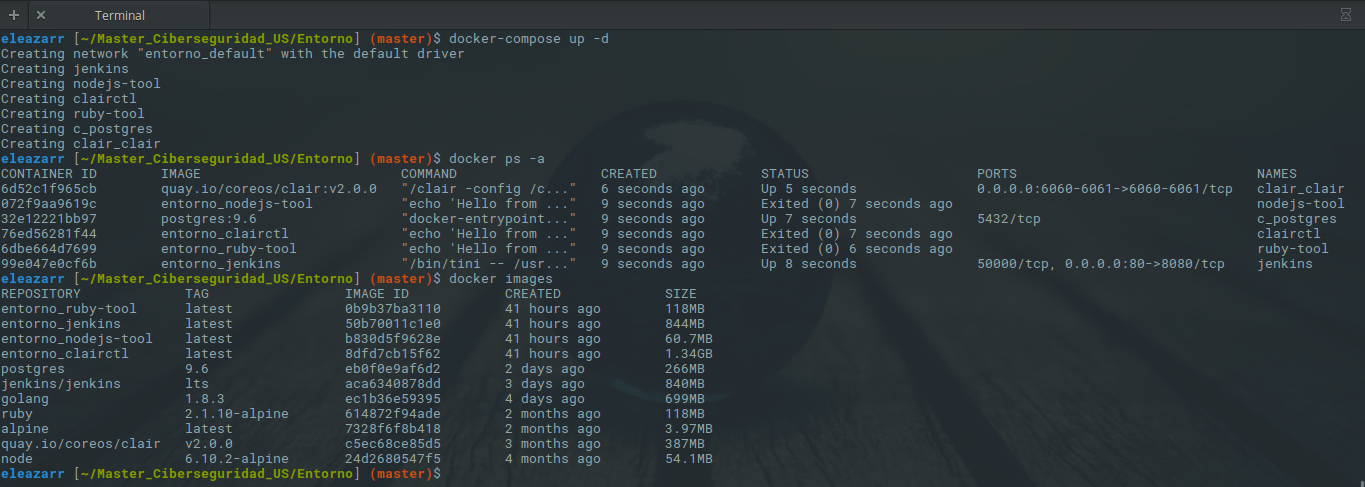
\includegraphics[width=1.0\linewidth]
	{desarrollo/figuras/docker-compose-up.png}
	\caption{Depliegue del entorno con Docker Compose}
	\label{compose}
\end{figure}

\subsection{Probando los componentes desplegados}

Ahora que todos los sistemas están funcionando en el sistema de contenedores es momento de comprobar que la configuración proporcionada es la correcta y que el comportamiento es el esperado. Para ello, y antes de automatizar las tareas con la ayuda de Jenkins, se van a realizar desde el interfaz de comandos las instrucciones necesarias que confirmen que los análisis se están llevando a cabo sin problema por parte de las herramientas de análisis.

El \autoref{prg04-05} muestra la ayuda aportada por el comando "docker exec", que será la utilidad proporcionada por Docker para la ejecución de instrucciones en el interior de los contenedores que se encuentran en ejecución en el entorno (Jenkins, clair\_clair y c\_postgres).

\begin{lstlisting}[language=,caption={Comando de ayuda de docker exec}, breaklines=true, label=prg04-05]
$ docker exec --help

Usage:	docker exec [OPTIONS] CONTAINER COMMAND [ARG...]

Run a command in a running container

Options:
	-d, --detach            Detached mode: run command in the background
	--detach-keys string   	Override the key sequence for detaching a container
	-e, --env list          Set environment variables
	--help                 	Print usage
	-i, --interactive       Keep STDIN open even if not attached
	--privileged           	Give extended privileges to the command
	-t, --tty               Allocate a pseudo-TTY
	-u, --user string       Username or UID (format: <name|uid>[:<group|gid>])
\end{lstlisting}

Para las imágenes de contenedores que no estén en ejecución Docker incluye la utilidad "docker run", con multitud de opciones y argumentos que se adaptan a las ejecuciones más variadas que puedan requerir las imágenes del sistema. El \autoref{prg04-05} ejemplifica el uso de la instrucción que será necesario llevar a cabo en el entorno actual presentado.

\begin{lstlisting}[language=,caption={Comando de ayuda de docker exec}, breaklines=true, label=prg04-06]
$ docker run --help

Usage:	docker run [OPTIONS] IMAGE [COMMAND] [ARG...]

...

$ sudo docker run --rm -t -i -v  ruta_local:ruta_contenedor imagen:tag /bin/bash
root@394bb66c4df0:/home/contenedor# pwd
/home/contenedor
\end{lstlisting}

Donde:

\begin{itemize}
	\item \textit{--rm} indica al demonio de Docker que una vez se termine de trabajar en el contenedor creado, este debe ser eliminado del sistema.
	\item \textit{-t -i} sirve para especificar que se va a abrir un terminal (-t) interactivo (-i) con el contenedor.
	\item \textit{-v} irá continuado por el volumen que se va a montar en el interior del contenedor de Docker.
	\item \textit{imagen:tag} será la imagen utilizada para crear el contenedor.
	\item \textit{/bin/bash} va a ser la instrucción ejecutada una vez creado el contenedor. Este comando va a devolver al usuario un terminal bash interactivo desde el interior del contenedor, donde poder ejecutar las instrucciones necesarias.
\end{itemize}

Conocidos estos comando y utilidades será posible comprobar la funcionalidad del sistema montado.

\subsubsection{Bundler Audit}

El \autoref{prg04-07} muestra los pasos a seguir para comprobar que Bundler Audit funciona correctamente desde el contenedor de Docker.

\begin{lstlisting}[language=,caption={Probando bundle-audit desde el contenedor}, breaklines=true, label=prg04-07]
eleazarr [~/Master_Ciberseguridad_US/Entorno] (master)$ docker run --rm -ti entorno_ruby-tool:latest sh

/ # curl https://raw.githubusercontent.com/EleazarWorkshare/gemfile_vulnerable/master/Gemfile.lock -o ./Gemfile.lock -s
/ # curl https://raw.githubusercontent.com/EleazarWorkshare/gemfile_vulnerable/master/Gemfile -o ./Gemfile -s

/ # bundle-audit check
Name: activesupport
Version: 4.1.1
Advisory: CVE-2015-3226
Criticality: Unknown
URL: https://groups.google.com/forum/#!topic/ruby-security-ann/7VlB_pck3hU
Title: XSS Vulnerability in ActiveSupport::JSON.encode
Solution: upgrade to >= 4.2.2, ~> 4.1.11

Name: activesupport
Version: 4.1.1
Advisory: CVE-2015-3227
Criticality: Unknown
URL: https://groups.google.com/forum/#!topic/rubyonrails-security/bahr2JLnxvk
Title: Possible Denial of Service attack in Active Support
Solution: upgrade to >= 4.2.2, ~> 4.1.11, ~> 3.2.22

Vulnerabilities found!

\end{lstlisting}

Analizando la ejecución en detalle:

\begin{enumerate}
	\item Se accede al contenedor que incluye la herramienta Bundle Audit.
	\item Mediante la \gls{API} de GitHub se descarga desde el repositorio que se quiere analizar los ficheros \textit{Gemfile} y \textit{Gemfile.lock} que incluyen las dependencias de la aplicación examinada.
	\item "bundle-audit check" examina los ficheros, descubriendo que existen vulnerabilidades en la versión 4.1.1 de la dependencia \textit{activesupport} contenida en el repositorio.
\end{enumerate}

\subsubsection{NSP}

El funcionamiento de nsp en el terminal de comando es muy similar al de bundler-audit, como demuestra la \autoref{nsp}.


\begin{figure}[htbp]
	\centering
	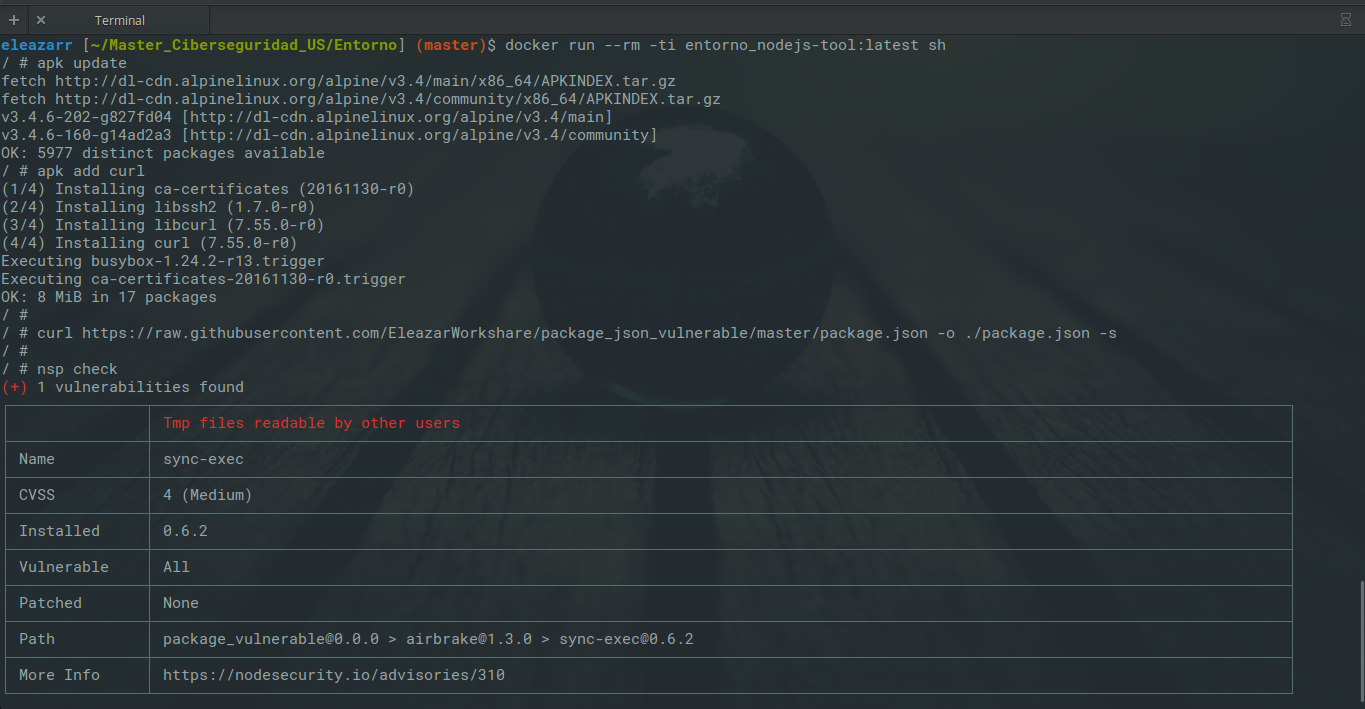
\includegraphics[width=1.0\linewidth]
	{desarrollo/figuras/nsp.png}
	\caption{Comprobando la utilidad nsp}
	\label{nsp}
\end{figure}

\TODO{UN PARRAFO MAS EXPLICANDO LA IMAGEN}

Con lo que queda demostrado que es posible desde el contenedor que ejecuta nsp acceder a la \gls{API} de GitHub, descargar un archivo \textit{package.json} con las dependencias de la aplicación node y realizar un análisis sobre este.

\subsubsection{Clair y Clairctl}

La forma de funcionamiento de Clairctl con Clair es diferente a las vistas para Bundler Audit y NSP, ya que Clairctl requiere de una configuración apropiada que le permita comunicarse con Clair y deberá realizar una serie de pasos para ello:

\begin{enumerate}
	\item Enviará la imagen que se quiere analizar a Clair para que la almacene (push). Dicha imagen podrá encontrarse en la máquina local que contiene a Clairctl o en un repositorio de imágenes de internet (pull).
	\item Clairctl pedirá a Clair que analiza la imagen enviada y le devuelva el resultado de dicho análisis (analyze).
	\item Clairctl generará un informe en formato HTML que podrá ser visualizado en el navegador del usuario.
\end{enumerate}

El proceso comentado se traduce en un mínimo de dos instrucciones de terminal para Clairctl: una para enviar y analizar la imagen en Clair y otra para realizar los informes. El \autoref{prg04-08} muestra el resultado de estas ejecuciones, tomando como ejemplo la propia imagen que contiene a Clairctl.

\begin{lstlisting}[language=,caption={Generando un informe HTML con Clairctl}, breaklines=true, label=prg04-08]
eleazarr [~/Master_Ciberseguridad_US/Entorno] (master)$ docker run --rm -ti -v /home/eleazarr/informe_clairctl:/go/src/github.com/jgsqware/clairctl/reports -v /var/run/docker.sock:/var/run/docker.sock:ro --net entorno_default --link clair_clair:clair -p 57330:57330 entorno_clairctl bash
root@59d0b5391fc6:/go# cd src/github.com/jgsqware/clairctl/
root@59d0b5391fc6:/go/src/github.com/jgsqware/clairctl# clairctl health

Clair: ✔

root@59d0b5391fc6:/go/src/github.com/jgsqware/clairctl# ./clairctl analyze --local entorno_clairctl:latest
2017-09-03 18:03:45.717118 I | config: retrieving interface for local IP
2017-09-03 18:03:45.717535 I | server: Starting Server on 172.20.0.4:57330
2017-09-03 18:03:45.722495 I | config: retrieving interface for local IP
2017-09-03 18:03:45.722730 I | clair: using http://172.20.0.4:57330/local as local url
2017-09-03 18:03:45.722748 I | clair: Pushing Layer 1/9 [b3ddc1248fc3]
2017-09-03 18:03:46.651866 I | clair: Pushing Layer 2/9 [b7f7dd16a445]
2017-09-03 18:03:46.654461 I | clair: Pushing Layer 3/9 [85ac2ce41a64]
2017-09-03 18:03:46.656823 I | clair: Pushing Layer 4/9 [089137f68fc4]
2017-09-03 18:03:46.658893 I | clair: Pushing Layer 5/9 [382f1b17bd70]
2017-09-03 18:03:46.660915 I | clair: Pushing Layer 6/9 [fef71688ca46]
2017-09-03 18:03:46.662980 I | clair: Pushing Layer 7/9 [71e3be3b4746]
2017-09-03 18:03:46.664839 I | clair: Pushing Layer 8/9 [76ceb8887997]
2017-09-03 18:03:46.666559 I | clair: Pushing Layer 9/9 [5ee4b01f03bd]
2017-09-03 18:03:46.668400 I | config: retrieving interface for local IP
2017-09-03 18:03:46.668611 I | clair: using http://172.20.0.4:57330/local as local url
2017-09-03 18:04:03.116083 I | clair: analysing layer [5ee4b01f03bd] 1/9
2017-09-03 18:04:03.143454 I | clair: analysing layer [76ceb8887997] 2/9
2017-09-03 18:04:03.190460 I | clair: analysing layer [71e3be3b4746] 3/9
2017-09-03 18:04:03.212756 I | clair: analysing layer [fef71688ca46] 4/9
2017-09-03 18:04:03.238765 I | clair: analysing layer [382f1b17bd70] 5/9
2017-09-03 18:04:03.285257 I | clair: analysing layer [089137f68fc4] 6/9
2017-09-03 18:04:03.302773 I | clair: analysing layer [85ac2ce41a64] 7/9
2017-09-03 18:04:03.316155 I | clair: analysing layer [b7f7dd16a445] 8/9
2017-09-03 18:04:03.325171 I | clair: analysing layer [b3ddc1248fc3] 9/9

Image: docker.io/entorno_clairctl:latest

Unknown: 15
Negligible: 65
Low: 49
Medium: 83
High: 37
Critical: 0
Defcon1: 0
root@59d0b5391fc6:/go/src/github.com/jgsqware/clairctl# ./clairctl report --local entorno_clairctl:latest                  

HTML report at ./reports/html/analysis-entorno_clairctl-latest.html
\end{lstlisting}

La \autoref{informe} muestra el resultado generado por Clairctl en el análisis de su propia imagen de Docker, confirmando que el sistema al completo se encuentra en perfecto estado de funcionamiento.

\begin{figure}[htbp]
	\centering
	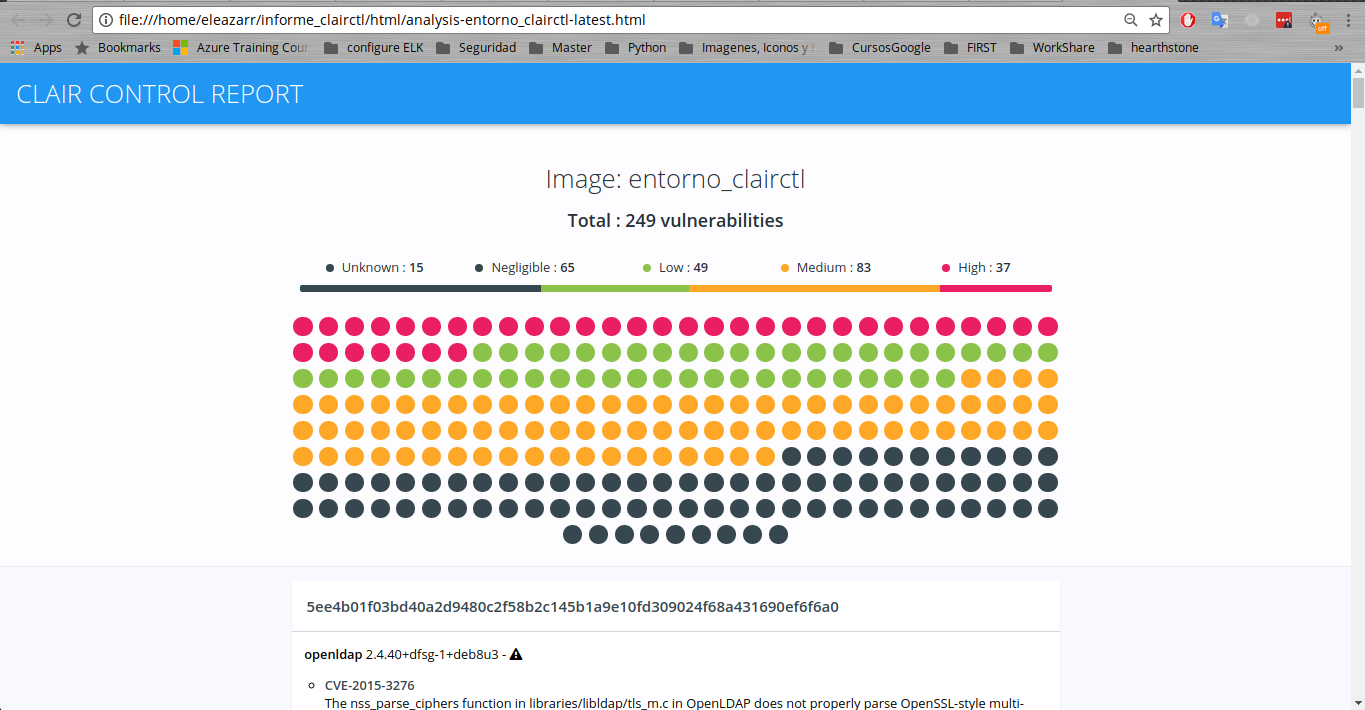
\includegraphics[width=1.0\linewidth]
	{desarrollo/figuras/informe_clairctl.png}
	\caption{Inorme generado por Clairctl}
	\label{informe}
\end{figure}

\subsubsection{Jenkins CI}

Para concluir el apartado se va a confirmar que existe el acceso apropiado al panel de trabajo de Jenkins, así como que se dispone de los plugins necesarios instalados para poder automatizar los trabajos de Jenkins, más conocidos por su traducción al inglés Jenkins Jobs.

En primer lugar, la \autoref{jenkins_01} muestra el mensaje de bienvenida que el usuario encontrará la primera vez que accede a la URL de la aplicación, solicitando un código oculto en el sistema de archivos de la misma. La \autoref{jenkins_02} muestra el acceso al código necesario para comenzar a crear el primer usuario de Jenkins.


\begin{figure}[htbp]
	\centering
	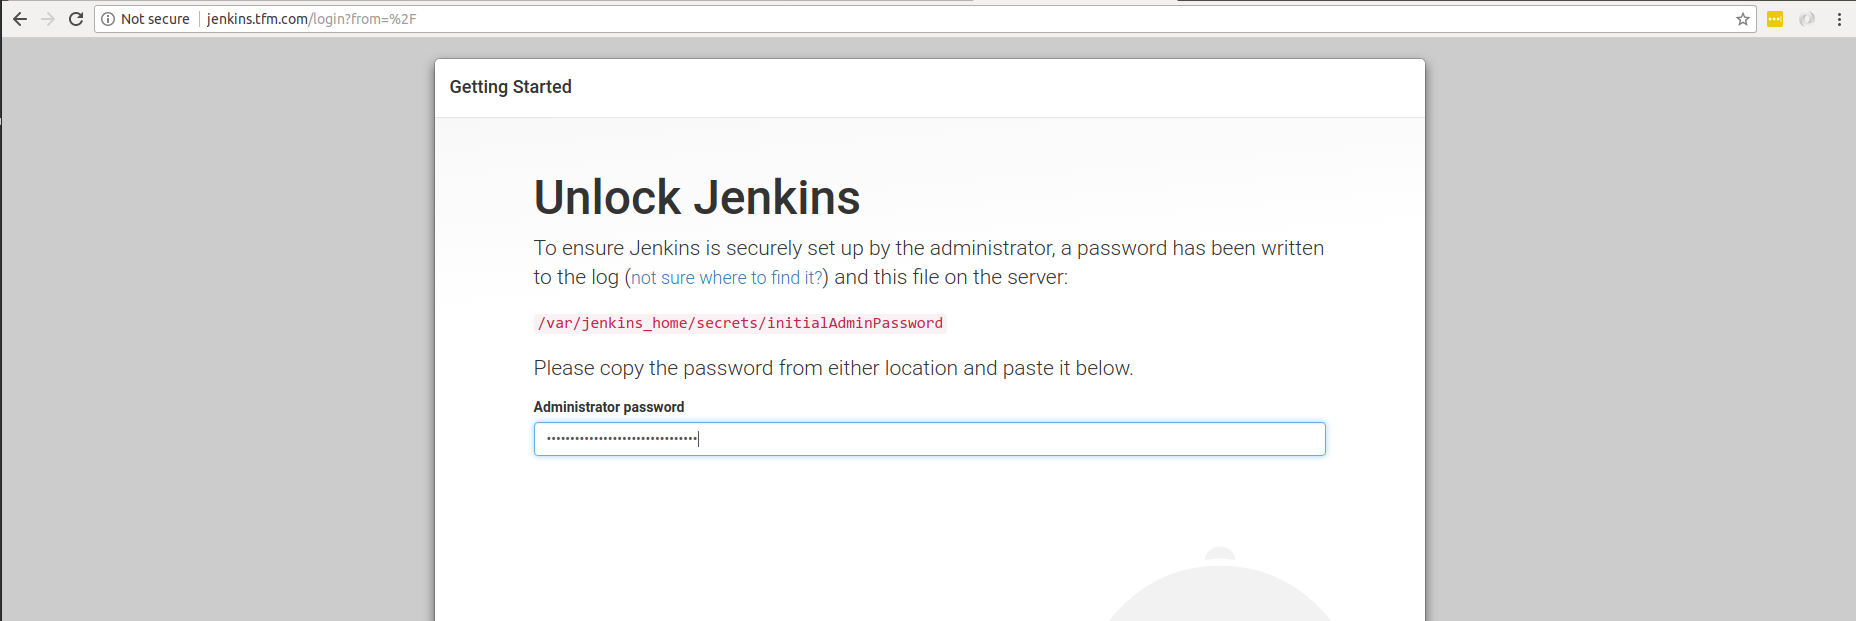
\includegraphics[width=1.0\linewidth]
	{desarrollo/figuras/jenkins_01.png}
	\caption{Bienvenida a la aplicación}
	\label{jenkins_01}
\end{figure}


\begin{figure}[htbp]
	\centering
	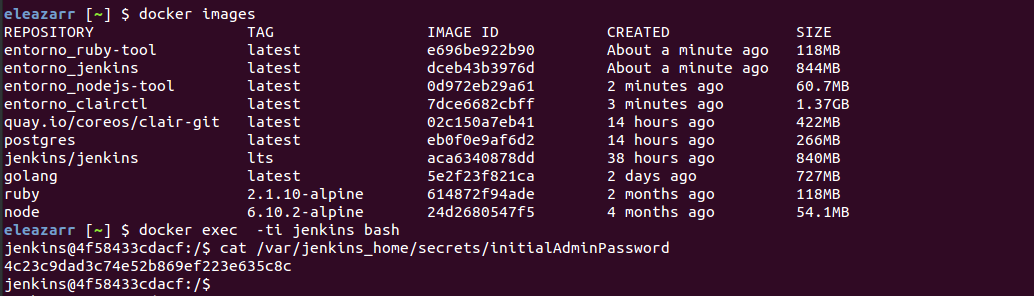
\includegraphics[width=1.0\linewidth]
	{desarrollo/figuras/jenkins_02.png}
	\caption{Encontrando el código oculto}
	\label{jenkins_02}
\end{figure}

Una vez superado la pantalla de bienvenida a la aplicación, se podrá decidir los plugins que serán instalados al inicio (\autoref{jenkins_03}) y comenzará el proceso de instalación inicial de plugins (\autoref{jenkins_04}).


\begin{figure}[htbp]
	\centering
	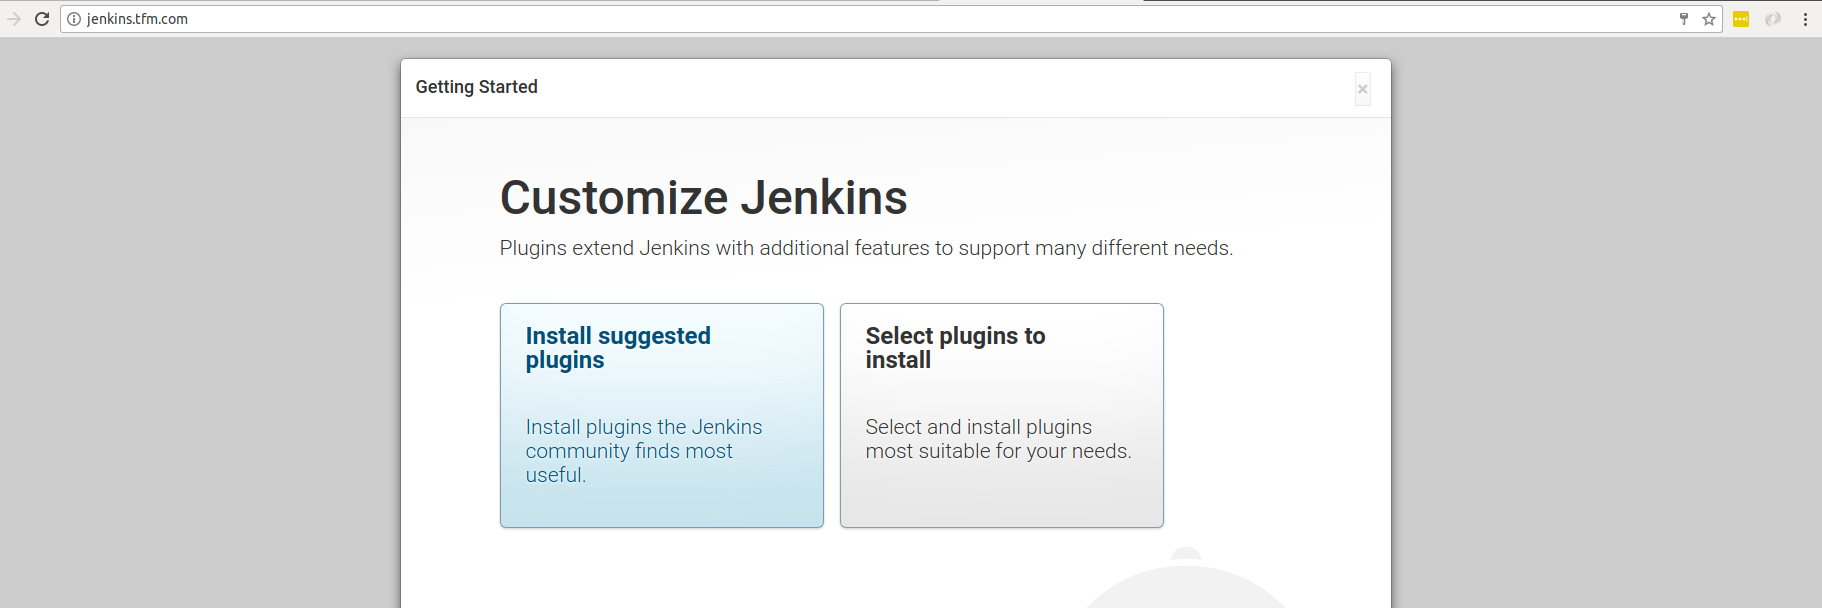
\includegraphics[width=1.0\linewidth]
	{desarrollo/figuras/jenkins_03.png}
	\caption{Instalando plugins recomendados}
	\label{jenkins_03}
\end{figure}

\begin{figure}[htbp]
	\centering
	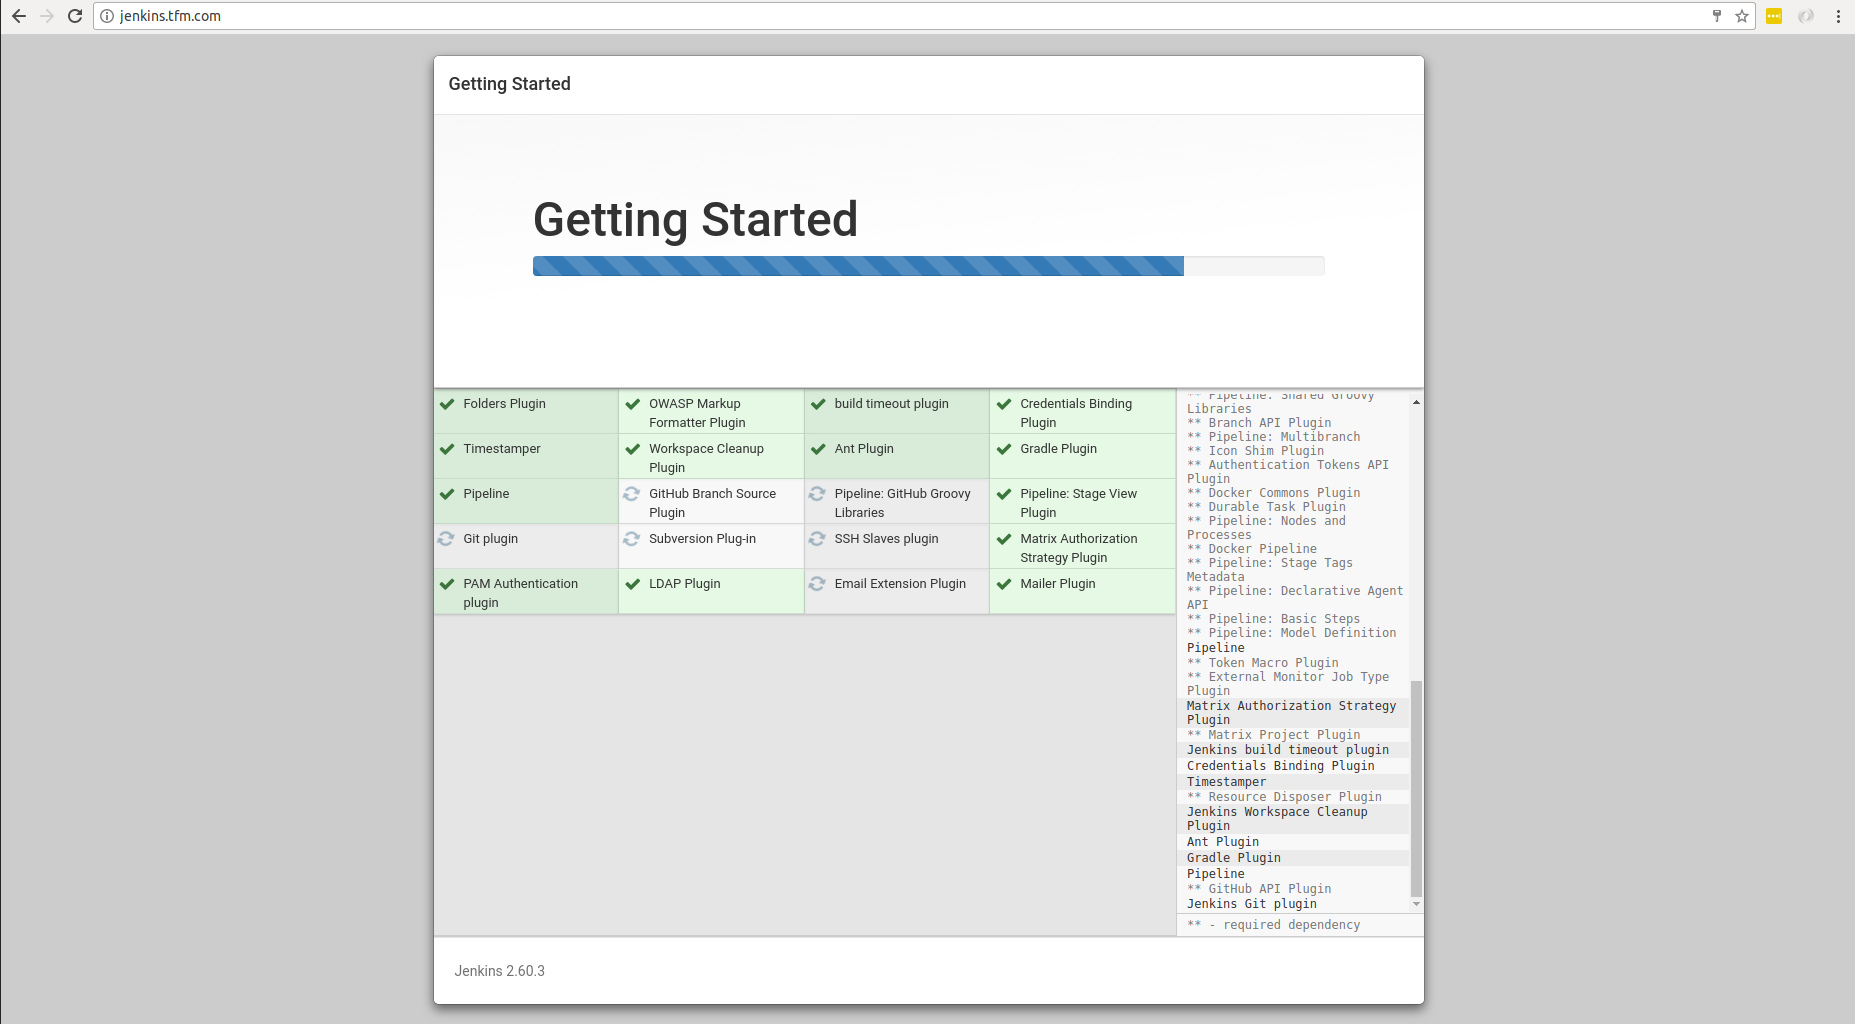
\includegraphics[width=1.0\linewidth]
	{desarrollo/figuras/jenkins_04.png}
	\caption{Proceso de instalación de plugins}
	\label{jenkins_04}
\end{figure}

El último paso de la preparación inicial será crear al primero de los usuarios administrador de la aplicación, la \autoref{jenkins_05} muestra al usuario creado.

\begin{figure}[htbp]
	\centering
	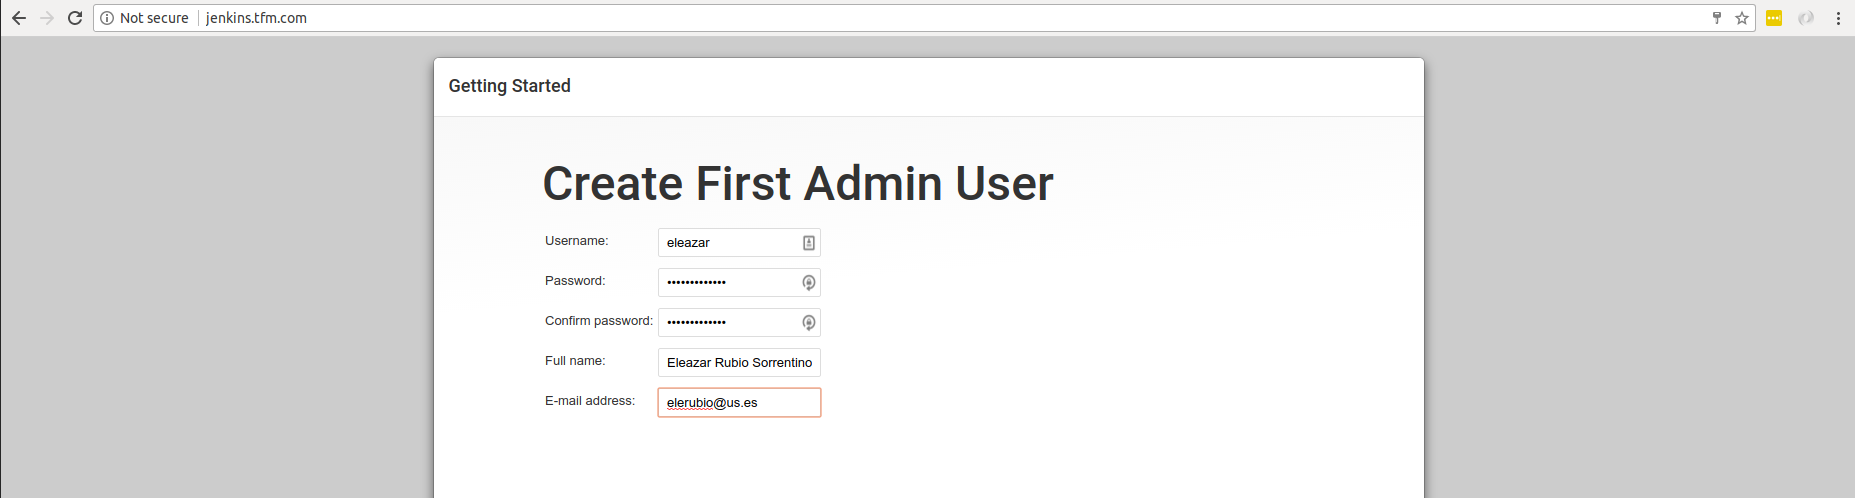
\includegraphics[width=1.0\linewidth]
	{desarrollo/figuras/jenkins_05.png}
	\caption{Creando el primer usuario administrador}
	\label{jenkins_05}
\end{figure}

Con esto la aplicación queda configurada y puede comenzar a usarse (\autoref{jenkins_06}).

\begin{figure}[htbp]
	\centering
	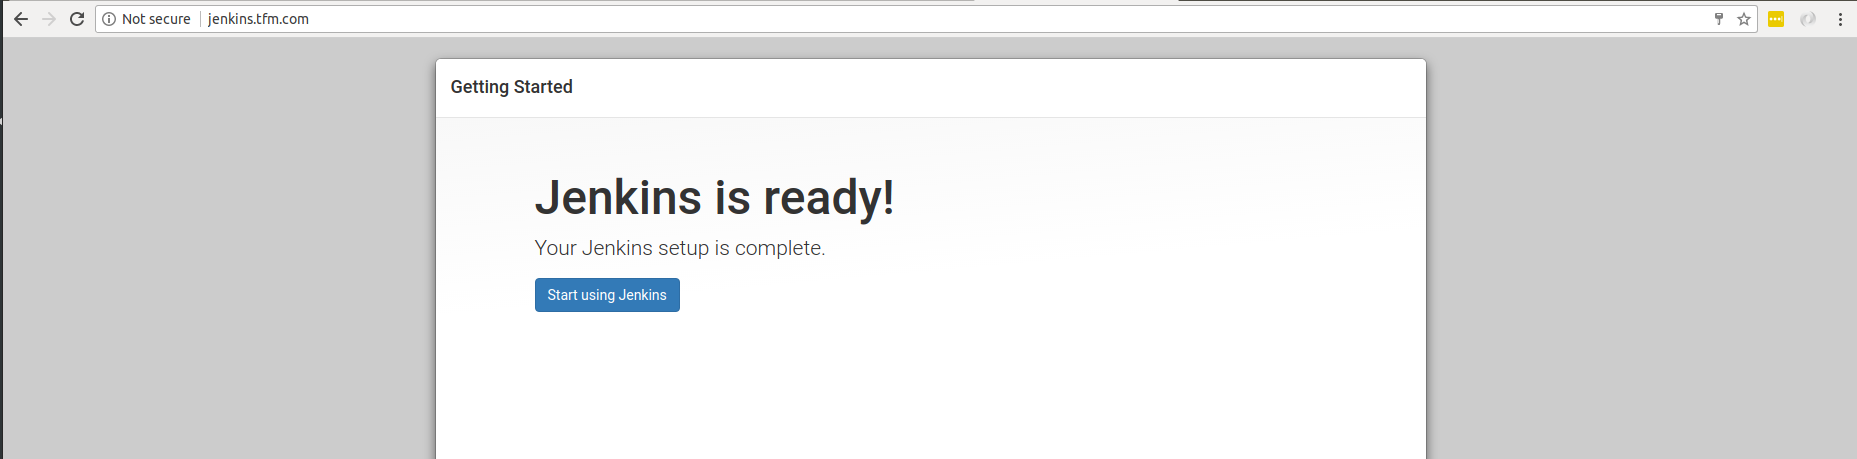
\includegraphics[width=1.0\linewidth]
	{desarrollo/figuras/jenkins_06.png}
	\caption{!Jenkins está listo!}
	\label{jenkins_06}
\end{figure}

Una vez Jenkins está configurado, lo primero que se deberá hacer para poder llevar a cabo el objetivo del presente \gls{TFM} será instalar el plugin \textit{HTML\_publisher}, puesto que será utilizando este como se crearán los informes HTML resultado de la ejecución de cada análisis estático. Las figuras \ref{jenkins_07} y \ref{jenkins_08} muestran las pantallas recorridas.

\begin{figure}[htbp]
	\centering
	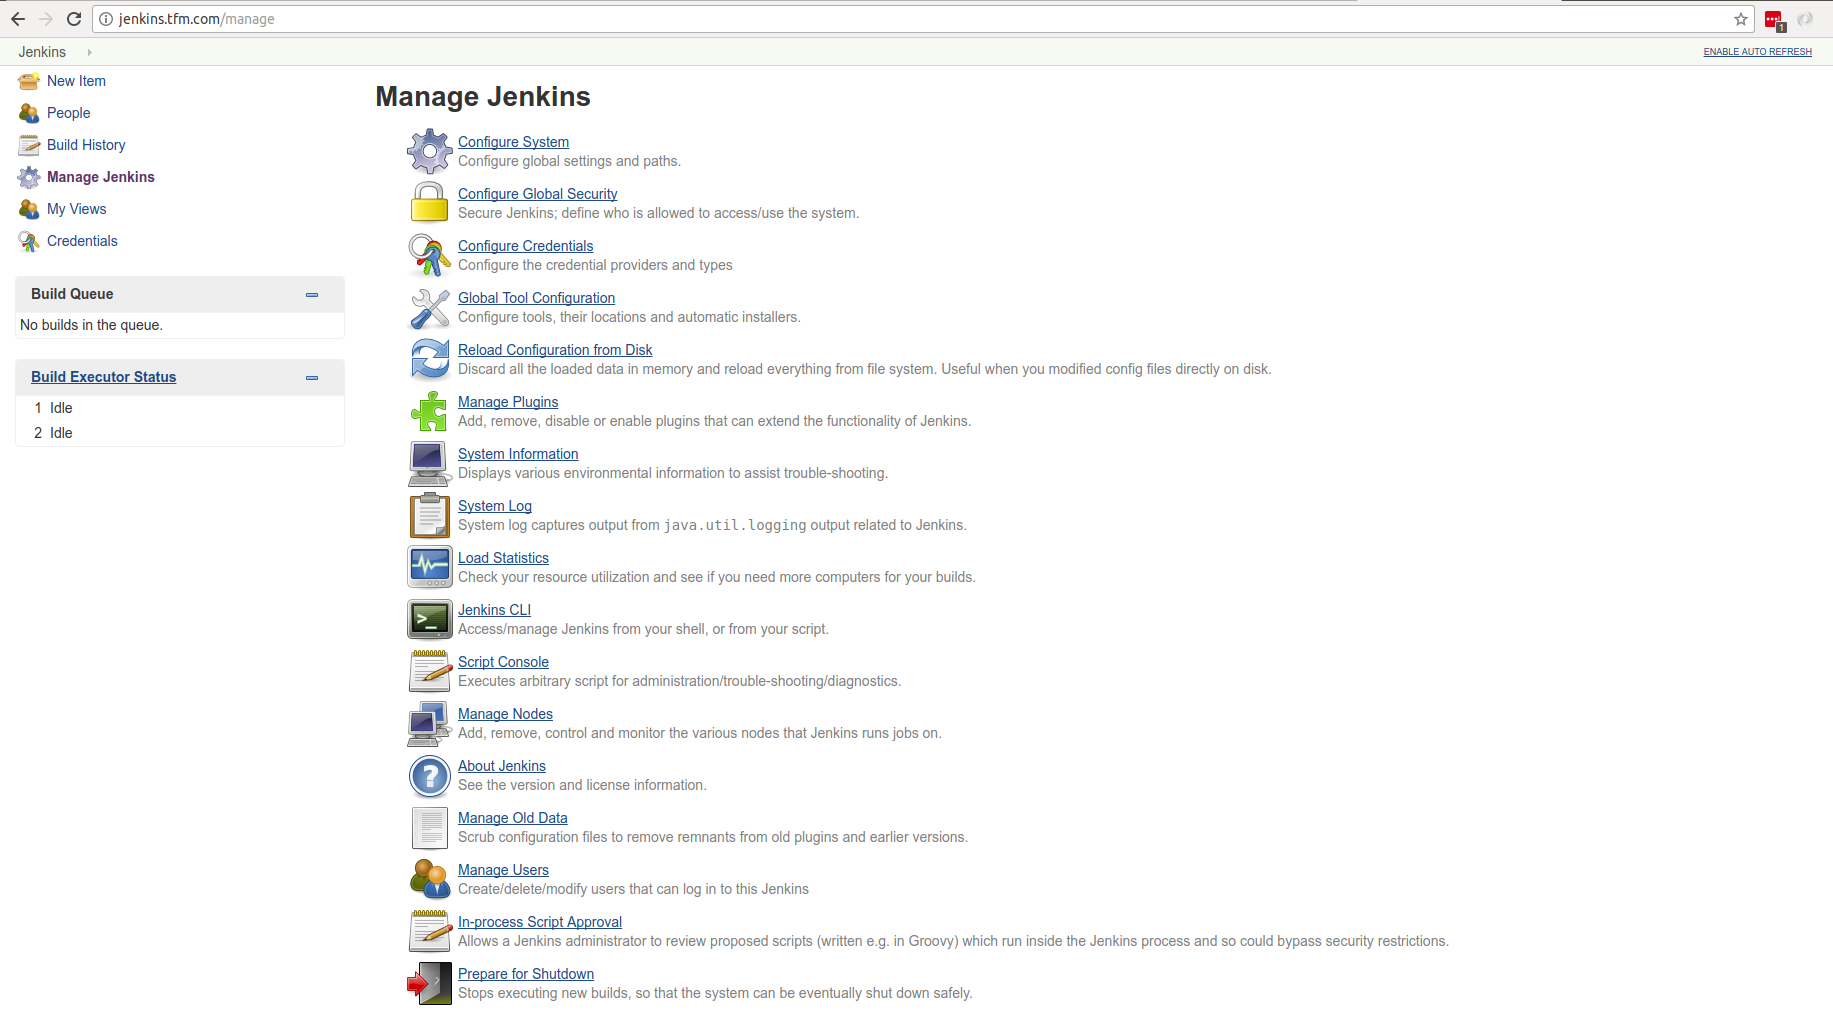
\includegraphics[width=1.0\linewidth]
	{desarrollo/figuras/jenkins_07.png}
	\caption{Manage Jenkins -> Manage Plugins}
	\label{jenkins_07}
\end{figure}

\begin{figure}[htbp]
	\centering
	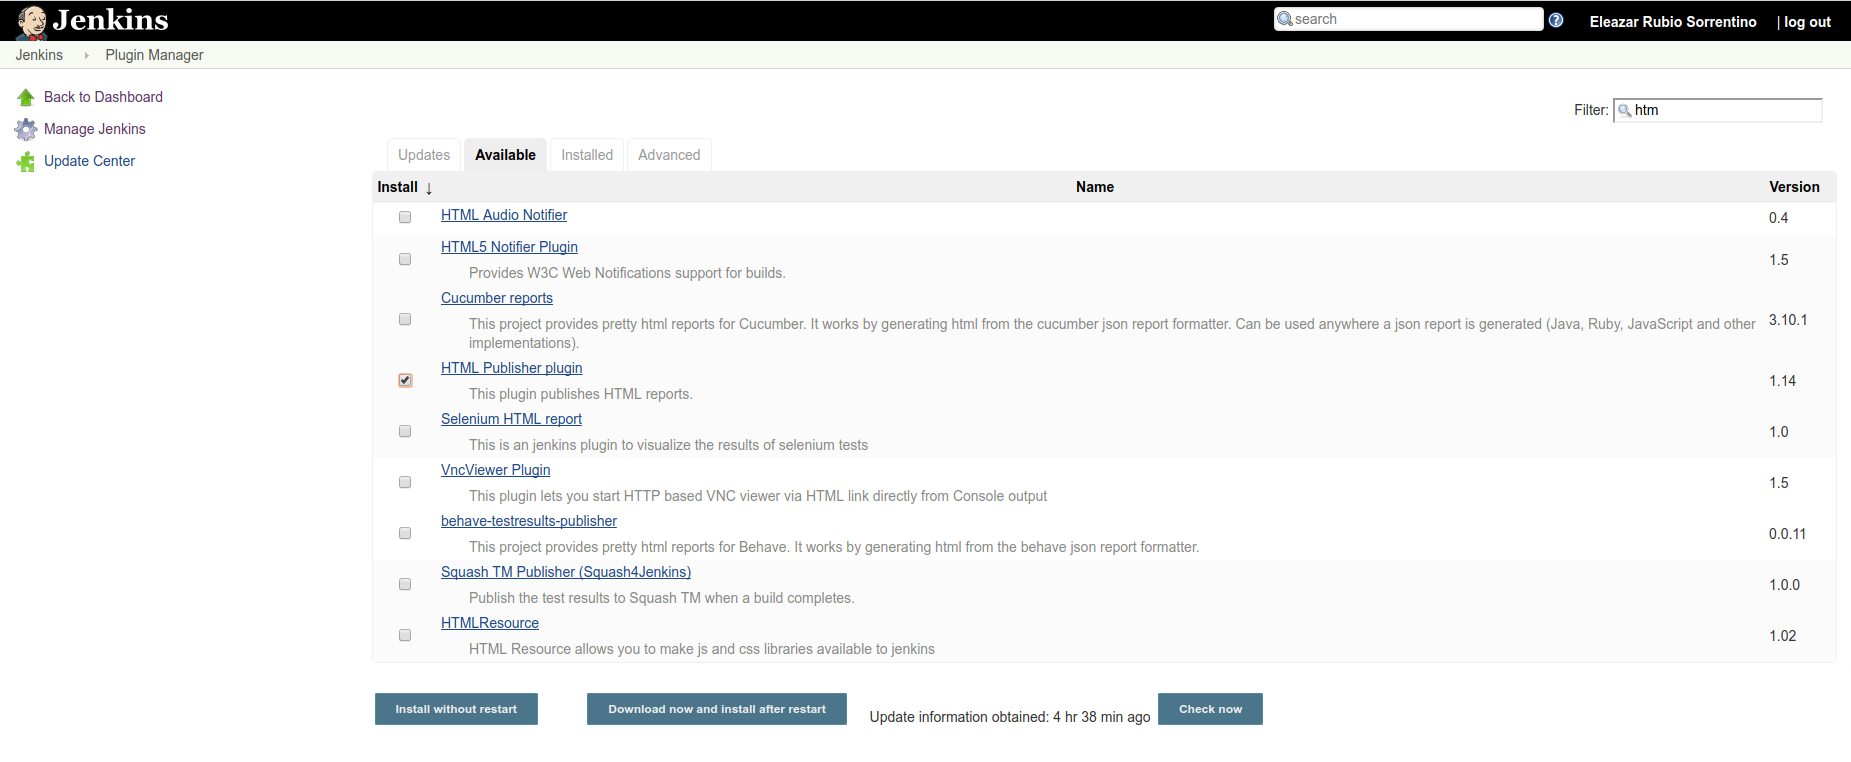
\includegraphics[width=1.0\linewidth]
	{desarrollo/figuras/jenkins_08.png}
	\caption{Instalando HTML\_publisher}
	\label{jenkins_08}
\end{figure}

Tras aplicar la instalación del plugin, y como muestra la \autoref{jenkins_09}, Jenkins se reiniciará, devolviendo al usuario al panel principal (\autoref{jenkins_10}) de la aplicación, con el entorno completamente configurado para comenzar a añadir los trabajos de Jenkins que automatizarán el proceso de análisis.

\begin{figure}[htbp]
	\centering
	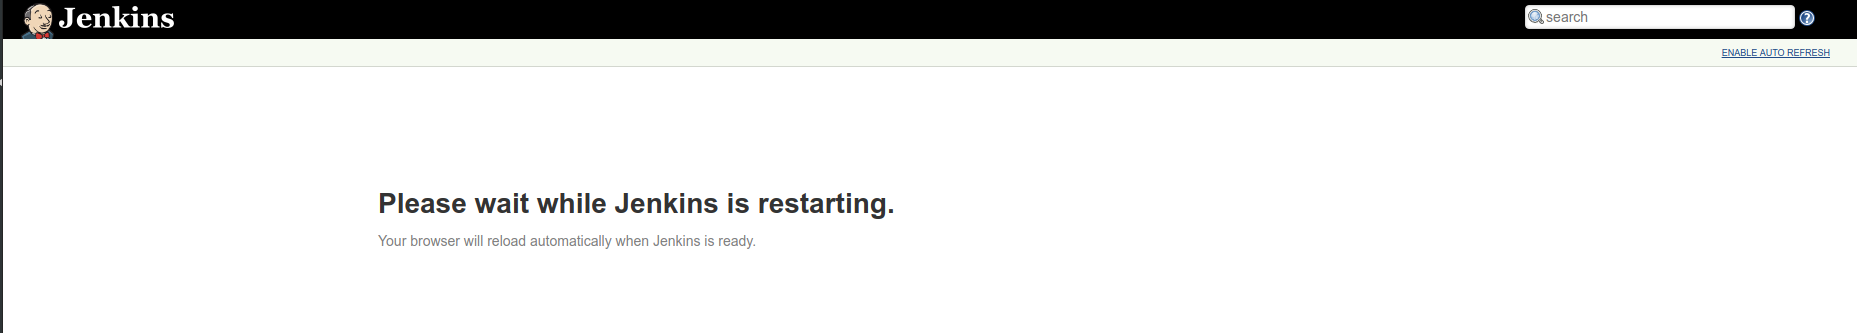
\includegraphics[width=1.0\linewidth]
	{desarrollo/figuras/jenkins_09.png}
	\caption{Reiniciando la aplicación tras la instalación del plugin}
	\label{jenkins_09}
\end{figure}

\begin{figure}[htbp]
	\centering
	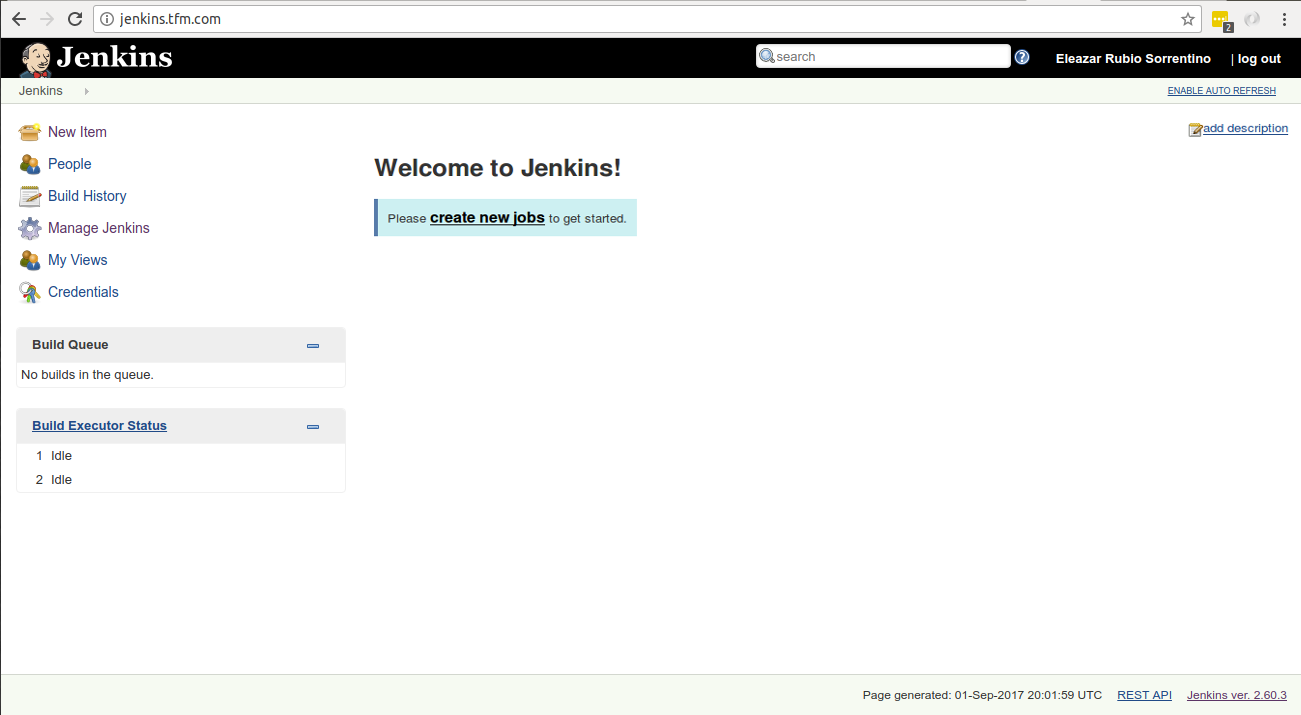
\includegraphics[width=1.0\linewidth]
	{desarrollo/figuras/jenkins_10.png}
	\caption{Pantalla de inicio de Jenkins \gls{CI}}
	\label{jenkins_10}
\end{figure}

\section{Trabajando con Jenkins}\label{trabajando_jenkins}

En la sección actual se va a utilizar el contenido empleado en los apartados de la \autoref{preparacion} para mostrar al lector la creación de tareas o trabajos en la plataforma de \gls{IC} Jenkins, con el fin de automatizar el proceso de análisis de las dependencias de código de aplicaciones escritas mediante los lenguajes de programación Ruby y Node.js, asi como el análisis de las posibles vulnerabilidades que pudieran mantener los contenedores de Docker utilizados por la compañía.

\subsection{Análisis de imágenes Docker}

\subsection{Análisis de dependencias Ruby}

\subsection{Análisis de de dependencias Node.js}

\section{Evaluación de la solución}

ALGUNAS EJECUCIONES QUE MUESTREN VULNERABILIDADES Y SOLUCIONAR ALGUNA.

\section{Resultados obtenidos}

CIERRE DEL APARTADO

\endinput

	
	%!TEX root =../MemoriaTFM.tex
%El anterior comando permite compilar este documento llamando al documento raíz
\chapter{Conclusiones}\label{chp-05}
\epigraph{Security is not a line in the sand. Protecting your business, customers, citizens’ data, should be always your number one priority}{Dr. Werner Vogels, 2017\\CTO at Amazon.com}

\lettrine[lraise=-0.1, lines=2, loversize=0.2]{E}{l} apartado actual, tras haber recorrido en la memoria de este \gls{TFM} "\eltitulo" toda la información relativa al proyecto, está dedicado a presentar los objetivos alcanzados y a presentar las líneas futuras de trabajo en torno al mismo. 

El conjunto de aplicaciones aportados a las herramientas y entorno utilizados surge ante la necesidad de las empresa moderna de vigilar de una manera no intrusiva los posibles agujeros y vulnerabilidades de seguridad que contengan las aplicaciones desarrolladas por ellas y los sistemas donde son desplegados. Esta tarea viene requiriendo un esfuerzo excesivo de parte de aquellas personas que se preocupan por mantener los sistemas lo más protegidos posible, aún cuando el ... puede estar originado en la multitud de dependencias que puede requerir una aplicación de gran envergadura o la inmensa cantidad de imágenes de diferente naturaleza que se despliegan en forma de contenedor en los entornos que dan soporte a las aplicaciones que sustentan el negocio.

Siguiendo esta ... se decide aportar al proceso de Integración Continua de empresas \gls{TI} un sencillo mecanismo de despliegue de contenedores que contendrán un conjunto de herramientas y utilidades con las que poder realizar tareas de análisis estático de manera pasiva como parte del proceso de trabajo natural de la compañía, analizando... , advirtiendo en caso de ... aportando ...\TODO{...}

Por este motivo se puede concluir que ... herramientas aportadas... junto con los trabajos automatizados... y ... cumple en conclusión con el objetivo perseguido en la realización de este \gls{TFM}.

Sin embargo, como es trivial en todo proceso tecnológico, la solución aquí entregada no es estática e inamovible y se presta a ser mejorada, además de a mantener los resultados obtenidos actualizados en el tiempo.

Muchas de las tareas y líneas de avance que este nuevo reto contempla aún son desconocidas, ya que van a surgir en la utilización por parte de los usuarios de la solución aportada. Otras, en cambio, pueden ser establecidas desde el momento actual. A continuación se presentan algunas de las tareas que conforman la línea futura de trabajo de esta aplicación, identificadas durante la realización del proyecto y la redacción de esta memoria:

\begin{itemize}
	\item Aumentar el número de lenguajes de programación contemplados en los análisis estáticos: existen múltiples herramientas en la actualidad de características similares a las aquí presentadas que cubren un amplio abanico de lenguajes de programación diferentes. Implementar un conjunto mayor de dichas herramientas como parte del conjunto actual es una notable mejora a lo aquí presentado.
	\item Sistema de notificaciones del resultado de los análisis:
	\item Preparación del entorno para el despliegue en producción:
	\item Ampliar los repositorios alcanzados:
\end{itemize}

Alcanzado este punto se puede concluir que, con este Trabajo Fin de Máster \gls{TFM}, se abarca un aspecto importante \TODO{...} seguridad en las tecnologías de la información\TODO{...} y la tarea de diaria de un experto en \TODO{...}: detección, estudio y solución a un problema de seguridad determinado, mediante la aplicación de la tecnología y los recursos disponibles.

Además, el resultado obtenido es un producto con utilidad tangible, que ya está siendo utilizado en los sistemas de Workshare Inc., proporcionando valor añadido a la actividad en materias de seguridad ... que allí se realiza y permitiendo \TODO{...}. Este aspecto es elemento clave a la hora de diferenciar el proyecto realizado, ya que existen múltiples trabajos realizados que nunca llegan a superar la barrera de estudios teóricos, para convertirse en un producto o herramienta final en completo funcionamiento, lo que sin duda es una enorme satisfacción para su autor.

\endinput

	
	%:Empieza todo lo que no constituye el cuerpo en si del libro.
	\backmatter
	
	%:Indice de figuras.
	\cleardoublepage
	\phantomsection
	
	%:Para añadir una línea en blanco en el TOC y separar esta lista
	\addtocontents{toc}{\protect\mbox{}\protect\hspace*{0pt}\par}
	\addcontentsline{toc}{listasb}{\listfigurename}
	\pagestyle{especial}
	\listoffigures
	
	%:Indice de tablas, coméntese las siguientes líneas si no se desea
	%:\cleardoublepage
	%:\phantomsection
	%:\addcontentsline{toc}{listasb}{\listtablename}
	%:\pagestyle{especial}
	%:\listoftables
	
	%:Indice de Código
	\cleardoublepage
	\phantomsection
	\addcontentsline{toc}{listasb}{\lstlistlistingname}
	\pagestyle{especial}
	\lstlistoflistings
	
	%:Bibliografía con biblatex y biber
	\cleardoublepage
	\phantomsection
	\addcontentsline{toc}{listasb}{\refname}
	\pagestyle{especial}
	%BIBER
	%\printbibliography[heading=etsi]z
	%BIBTEX
	%\bibliographystyle{IEEEtran}
	\bibliographystyle{amsplain} %flexbib amsplain alpha
	%:Fichero con la bibliografía, BIBTEX
	\bibliography{bibliografia}
	
	
	%:Acrónimos
	\cleardoublepage
	\phantomsection
	\addcontentsline{toc}{listasb}{\glossaryname}
	\chaptermark{\glossaryname}
	\printglossary[type=\acronymtype,title=Glosario]
	
\end{document}